%Motivation:
%%%%%%%%%%%%%%%%%%%%%%%%%%%%%%%%%%%%%%%%%%%%%%%%%%
\begin{frame}[fragile]{}

\begin{center}
{
\LARGE
\de{Warum}\en{Why} Domain-Driven Design?
}
\end{center}

\end{frame}

%%%%%%%%%%%%%%%%%%%%%%%%%%%%%%%%%%%%%%%%%%%%%%%%%%
\begin{frame}[fragile]{DDD in a Nutshell}

\begin{itemize}
\item \de{Gemeinsames Verständnis schaffen}\en{Build common understanding}
\item \de{Trennung Business Logik $\leftrightarrow$ Technik}\en{Separate business logic $\leftrightarrow$ technical stuff}
\item \de{Strukturierung des Codes}\en{Structure the code}
\end{itemize}

\end{frame}

%-----------------------------------------------------------------------------------------------------------------------------------
\numberednote{

Wir fokussieren heute auf den 1. und ein Stück weit auf den 2. Aspekt.
}

%%%%%%%%%%%%%%%%%%%%%%%%%%%%%%%%%%%%%%%%%%%%%%%%%%
\begin{frame}[fragile]{\de{Gemeinsames Verständnis schaffen}\en{Build Common Understanding}}

\begin{itemize}
\item \de{Hat hohen Stellenwert}\en{Very important}
\item \glqq Knowledge Crunching\grqq
\end{itemize}

\end{frame}

%Wurde lange Zeit ein bisschen hand-wavey betrachtet: "dann macht man das und dann bekommt man ein gutes Modell"
%%%%%%%%%%%%%%%%%%%%%%%%%%%%%%%%%%%%%%%%%%%%%%%%%%
\begin{frame}[fragile]{}

 \begin{tikzpicture}
 % x (kleiner = weiter nach links) y (kleiner = weiter nach unten)
             \put (3,-157.3) 
             { 
\includegraphics[height=\paperheight]{pics/do-knowledge-crunching-and-all-will-be-well.jpg} };
\end{tikzpicture}

\end{frame}

%%%%%%%%%%%%%%%%%%%%%%%%%%%%%%%%%%%%%%%%%%%%%%%%%%
\begin{frame}[fragile]{}

 \begin{tikzpicture}
 % x (kleiner = weiter nach links) y (kleiner = weiter nach unten)
             \put (28,-157.3) 
{ 
\includegraphics[height=\paperheight]{pics/one-does-not-simply-do-knowledge-crunching.jpg} };
\end{tikzpicture}

\end{frame}

%Dann kam EventStorming auf den Plan
%%%%%%%%%%%%%%%%%%%%%%%%%%%%%%%%%%%%%%%%%%%%%%%%%%
\begin{frame}[fragile]{}

 \begin{tikzpicture}
 % x (kleiner = weiter nach links) y (kleiner = weiter nach unten)
            \put (-10,10) { 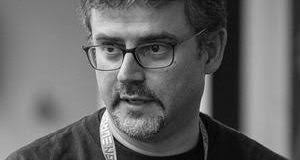
\includegraphics[width=.5\textwidth]{pics/alberto_brandolini.jpg} };
\end{tikzpicture}

\onslide+<2->
 \begin{tikzpicture}
            \put (100,-80) { 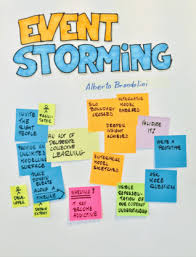
\includegraphics[height=.5\textheight]{pics/eventstorming.jpg} };
\end{tikzpicture}

\onslide+<3->
 \begin{tikzpicture}
            \put (180,-120) { 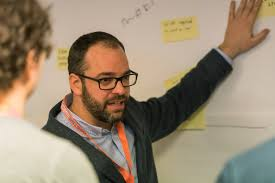
\includegraphics[width=.5\textwidth]{pics/mathias_verraes.jpg} };
\end{tikzpicture}

\end{frame}

%-----------------------------------------------------------------------------------------------------------------------------------
\numberednote{

Standing on the shoulders of giants

~\\

Das möchte ich Euch heute vorstellen

\begin{itemize}
\item Wenig Domain-Driven Design
\item Viel gemeinsames Verständnis
\begin{itemize}
\item Knowledge Crunching
\item mit EventStorming
\end{itemize}
\end{itemize}

EventStorming: sehr schnell sehr detailliertes Modell
}


%%%%%%%%%%%%%%%%%%%%%%%%%%%%%%%%%%%%%%%%%%%%%%%%%%
\begin{frame}[fragile]{\de{Gemeinsames Verständnis schaffen - Warum?}\en{Create Common Understanding - Why?}}

\begin{itemize}
\item \de{Gedanken sichtbar und ``begreifbar'' machen}\en{Make thoughts visible and tangible}
\item \de{Modell schafft Klarheit}\en{Model establishes clarity}
\item Ubiquitous Language \de{grenzt Begriffe ab}\en{defines the scope of terms}
\end{itemize}

\end{frame}

%-----------------------------------------------------------------------------------------------------------------------------------
\numberednote{

Jeder entwickelt eigene Vorstellung von etwas Gehörtem

}

%%%%%%%%%%%%%%%%%%%%%%%%%%%%%%%%%%%%%%%%%%%%%%%%%%
\begin{frame}[fragile]{}

 \begin{tikzpicture}
 % x (kleiner = weiter nach links) y (kleiner = weiter nach unten)
             \put (-50,-167.3) 
{ 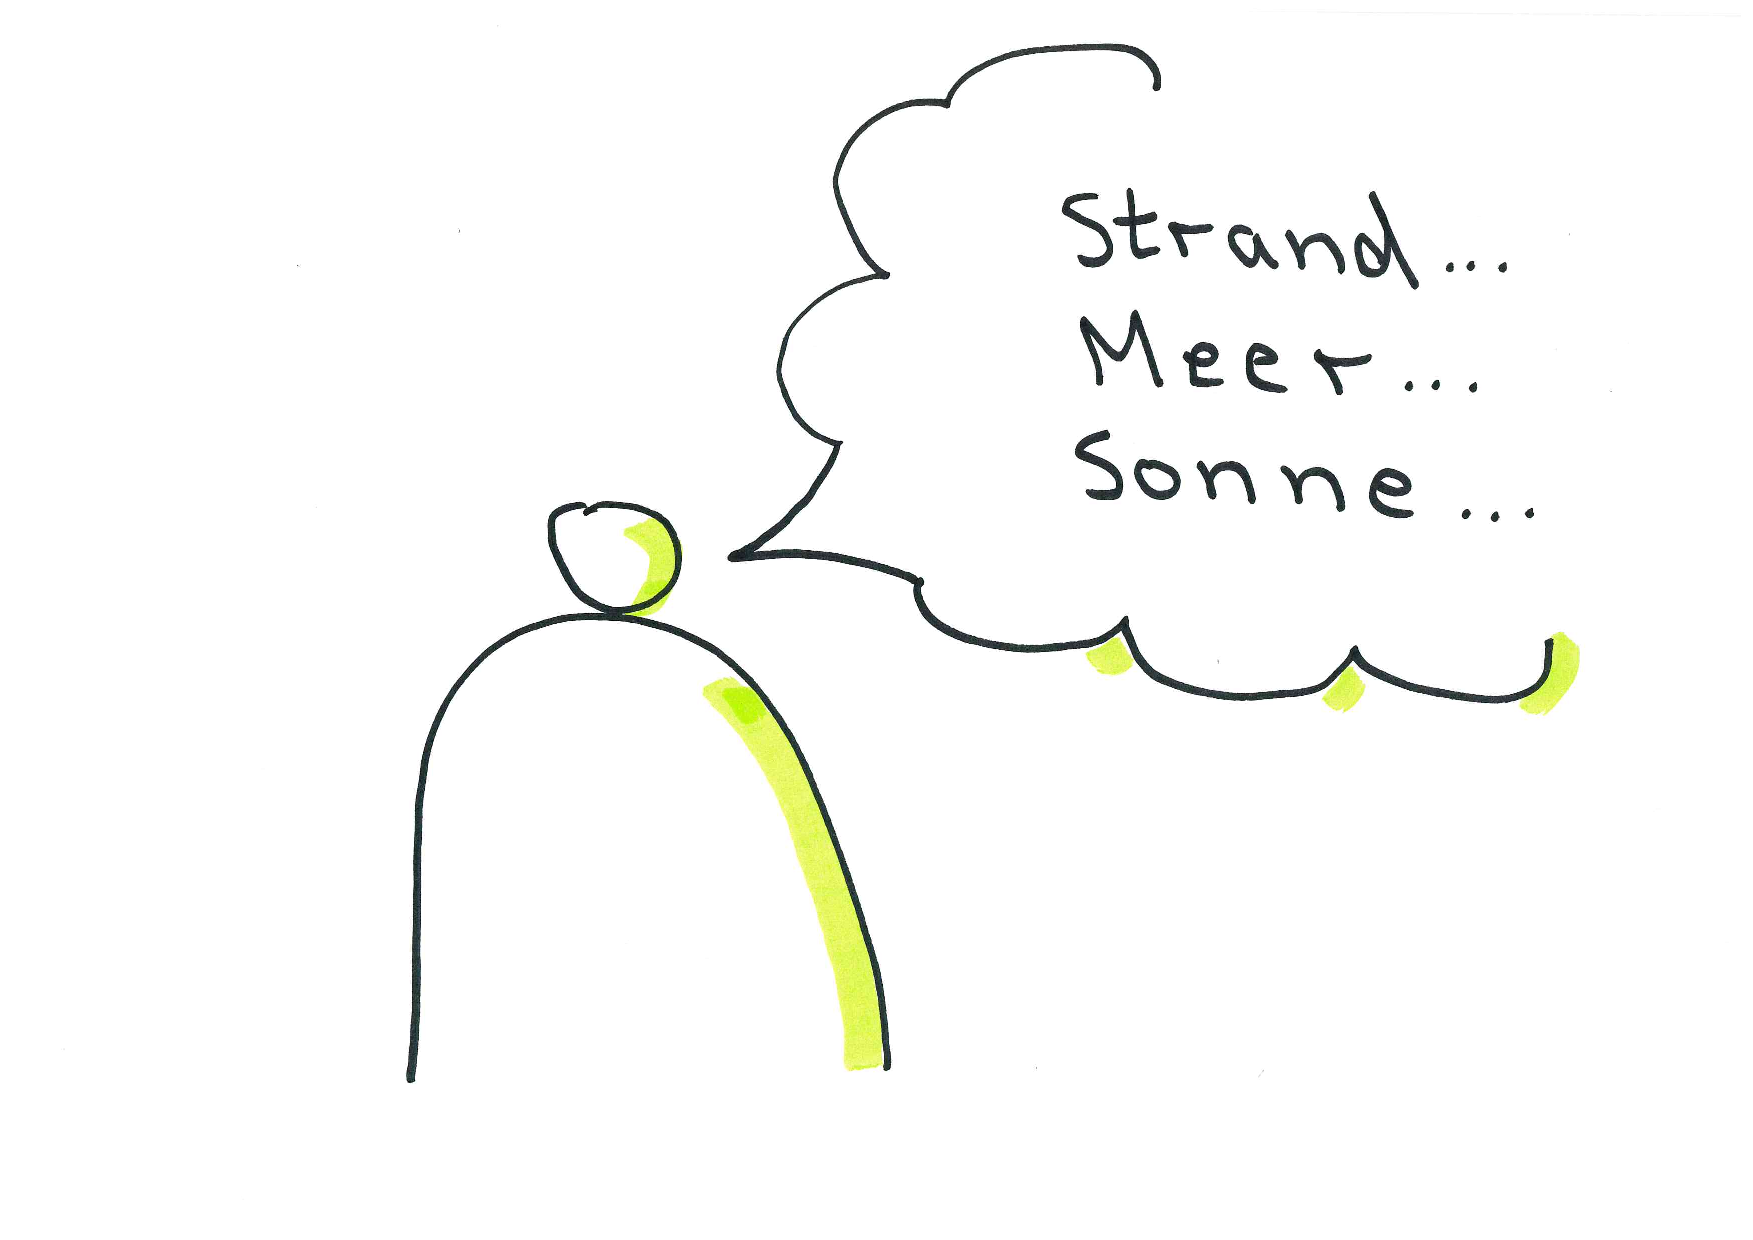
\includegraphics[height=\paperheight]{pics/ich_berichte_von_meinem_urlaub.pdf} % sonne, strand, meer
};
\end{tikzpicture}

\end{frame}

%-----------------------------------------------------------------------------------------------------------------------------------
\numberednote{

\begin{itemize}
\item strand breitete sich vor mir aus, meer schwappte sanft ans ufer, sonne stand am himmel
\item jeder von euch hat wahrscheinlich ein bild im kopf
\item vielleicht sieht euer bild so oder so ähnlich aus
\item vielleicht war ich aber gar nicht allein, sondern in Gesellschaft
\item vielleicht war ich auch in einem anderen kulturkreis
\item oder vielleicht in einer anderen Klimazone
\end{itemize}

auf alle diese bilder passt die beschreibung von sonne, strand und meer

}


%%%%%%%%%%%%%%%%%%%%%%%%%%%%%%%%%%%%%%%%%%%%%%%%%%
\begin{frame}[fragile]{}

 \begin{tikzpicture}
 % x (kleiner = weiter nach links) y (kleiner = weiter nach unten)
             \put (-15,-157.3) 
{ 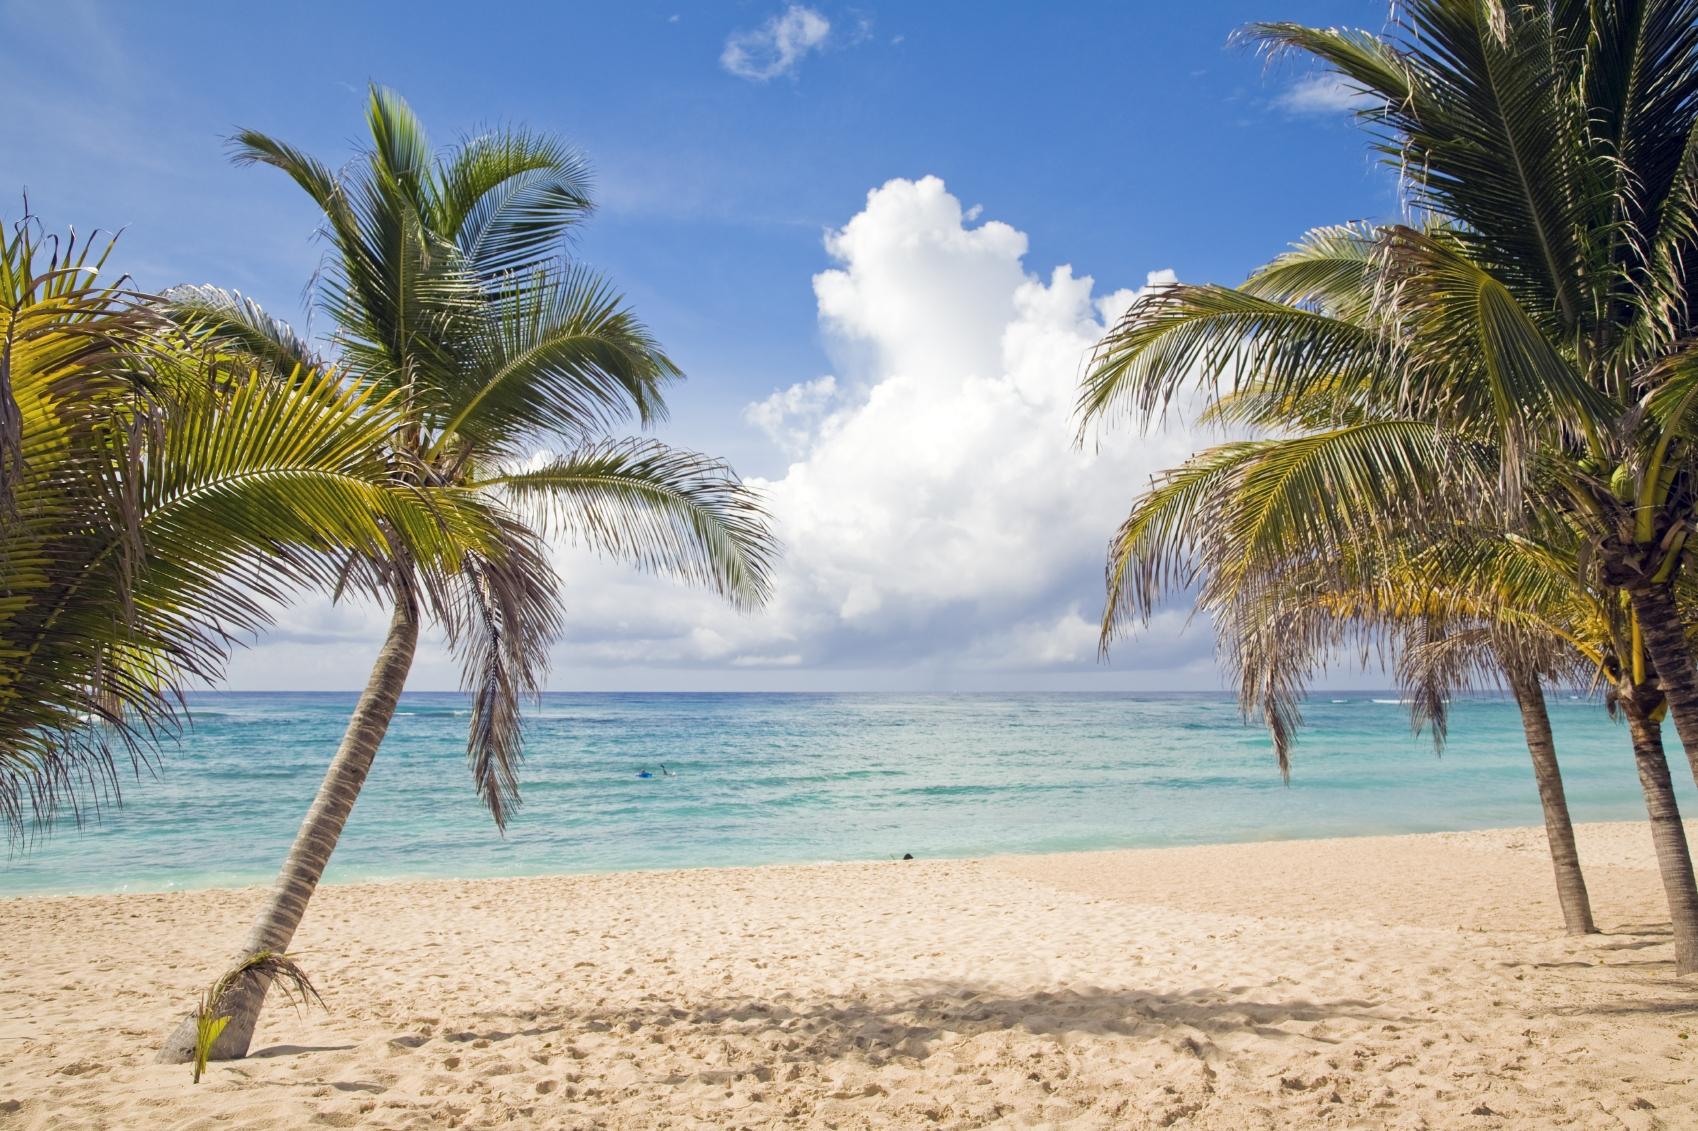
\includegraphics[height=\paperheight]{pics/palm_beach.jpg}
            };
\end{tikzpicture}

\end{frame}

%%%%%%%%%%%%%%%%%%%%%%%%%%%%%%%%%%%%%%%%%%%%%%%%%%
\begin{frame}[fragile]{}

 \begin{tikzpicture}
 % x (kleiner = weiter nach links) y (kleiner = weiter nach unten)
             \put (-15,-157.3) 
{ 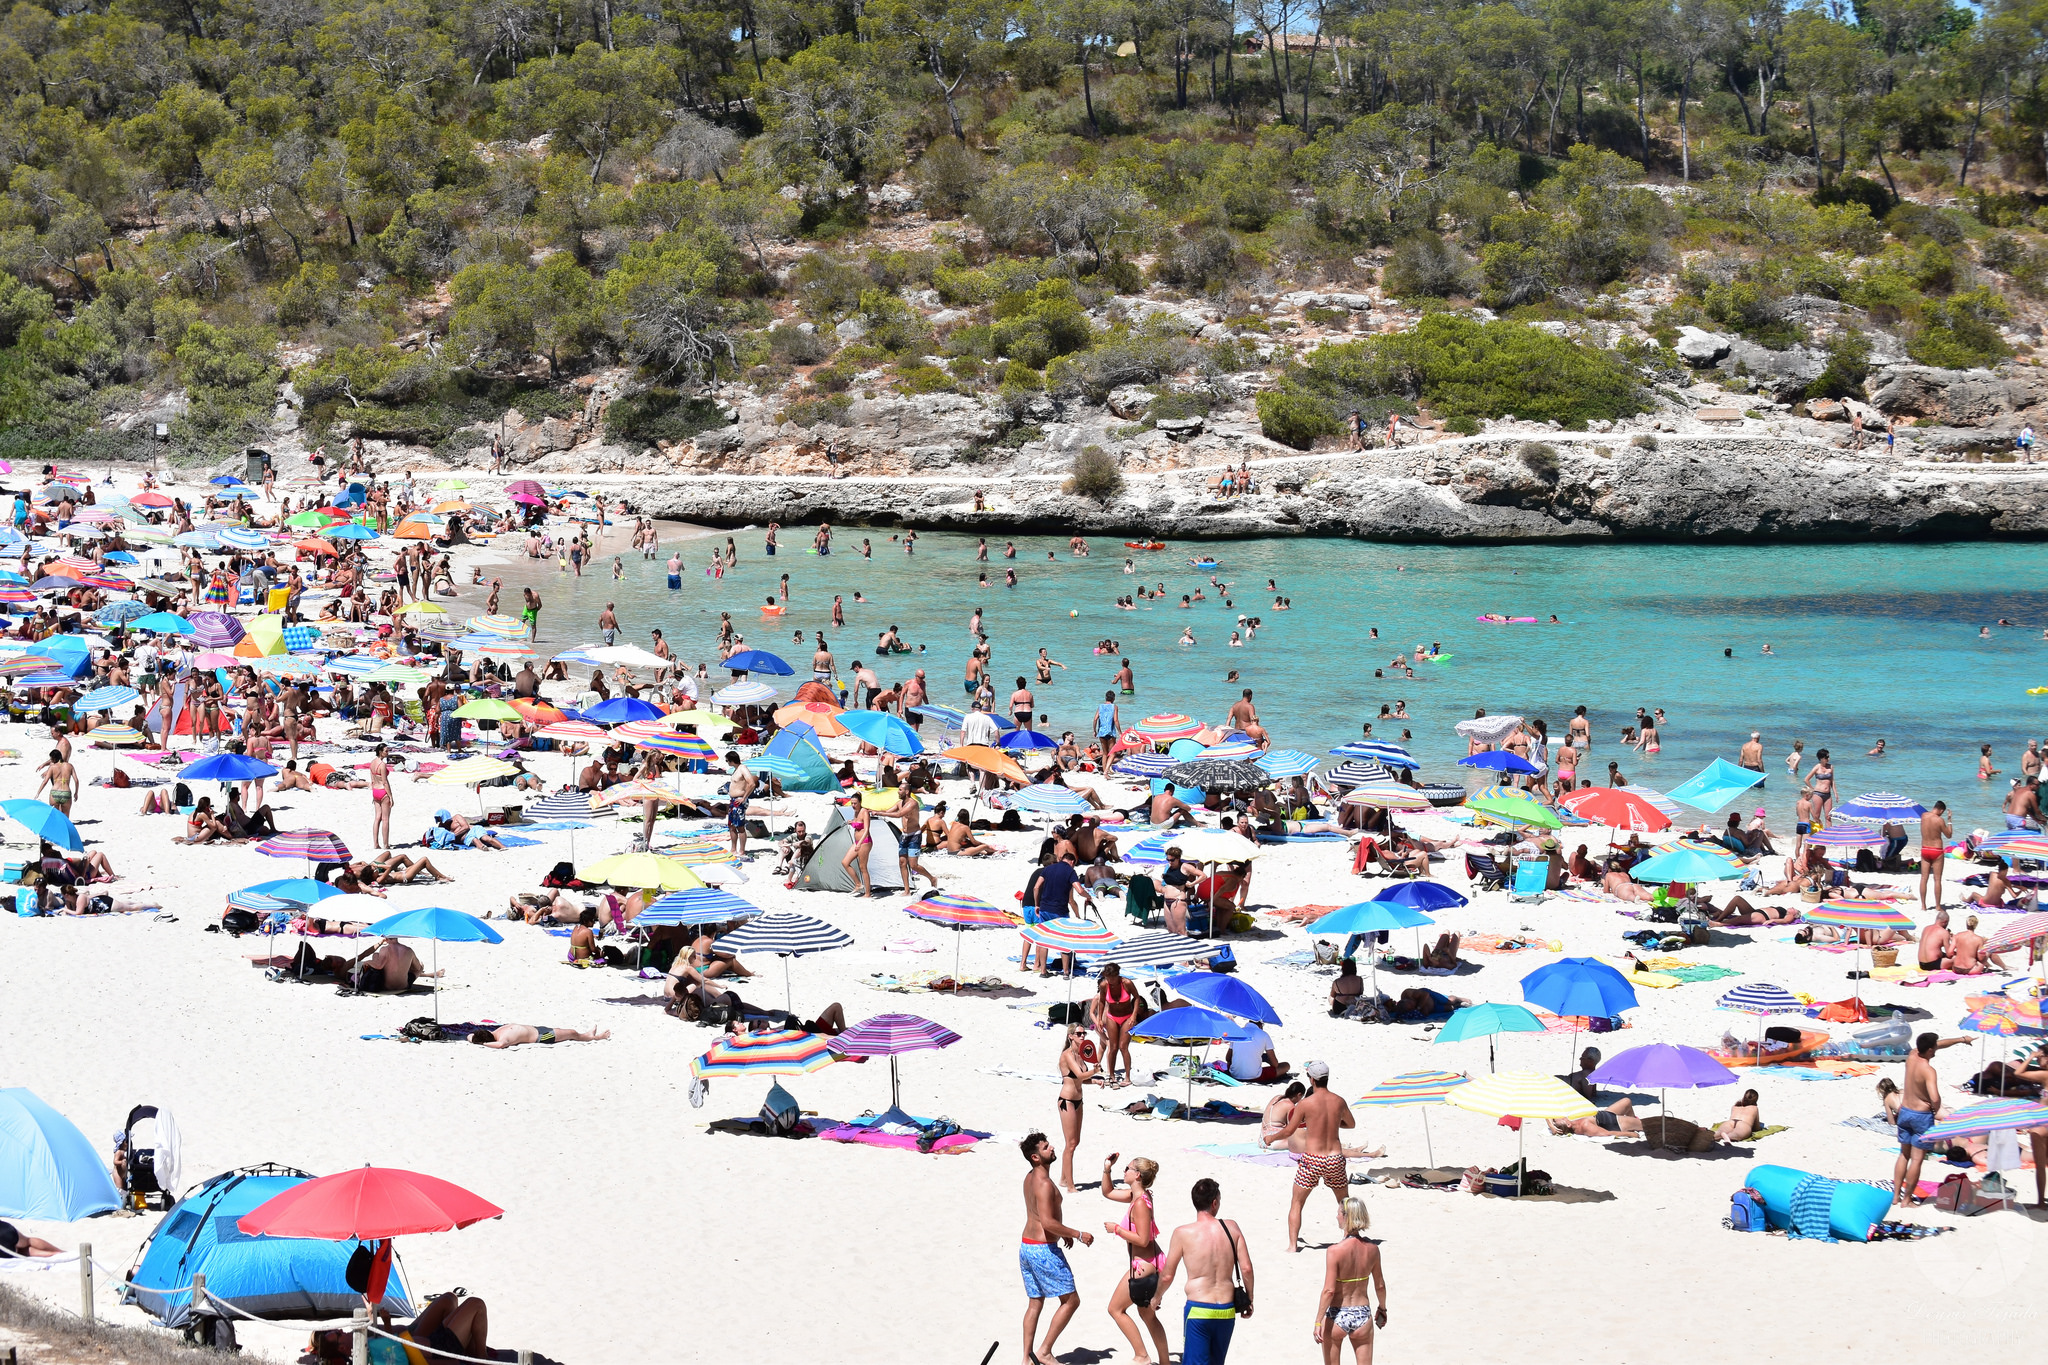
\includegraphics[height=\paperheight]{pics/mallorca_beach.jpg}
            };
\end{tikzpicture}

\end{frame}

%%%%%%%%%%%%%%%%%%%%%%%%%%%%%%%%%%%%%%%%%%%%%%%%%%
\begin{frame}[fragile]{}

 \begin{tikzpicture}
 % x (kleiner = weiter nach links) y (kleiner = weiter nach unten)
             \put (-14.2,-157.3) 
{ 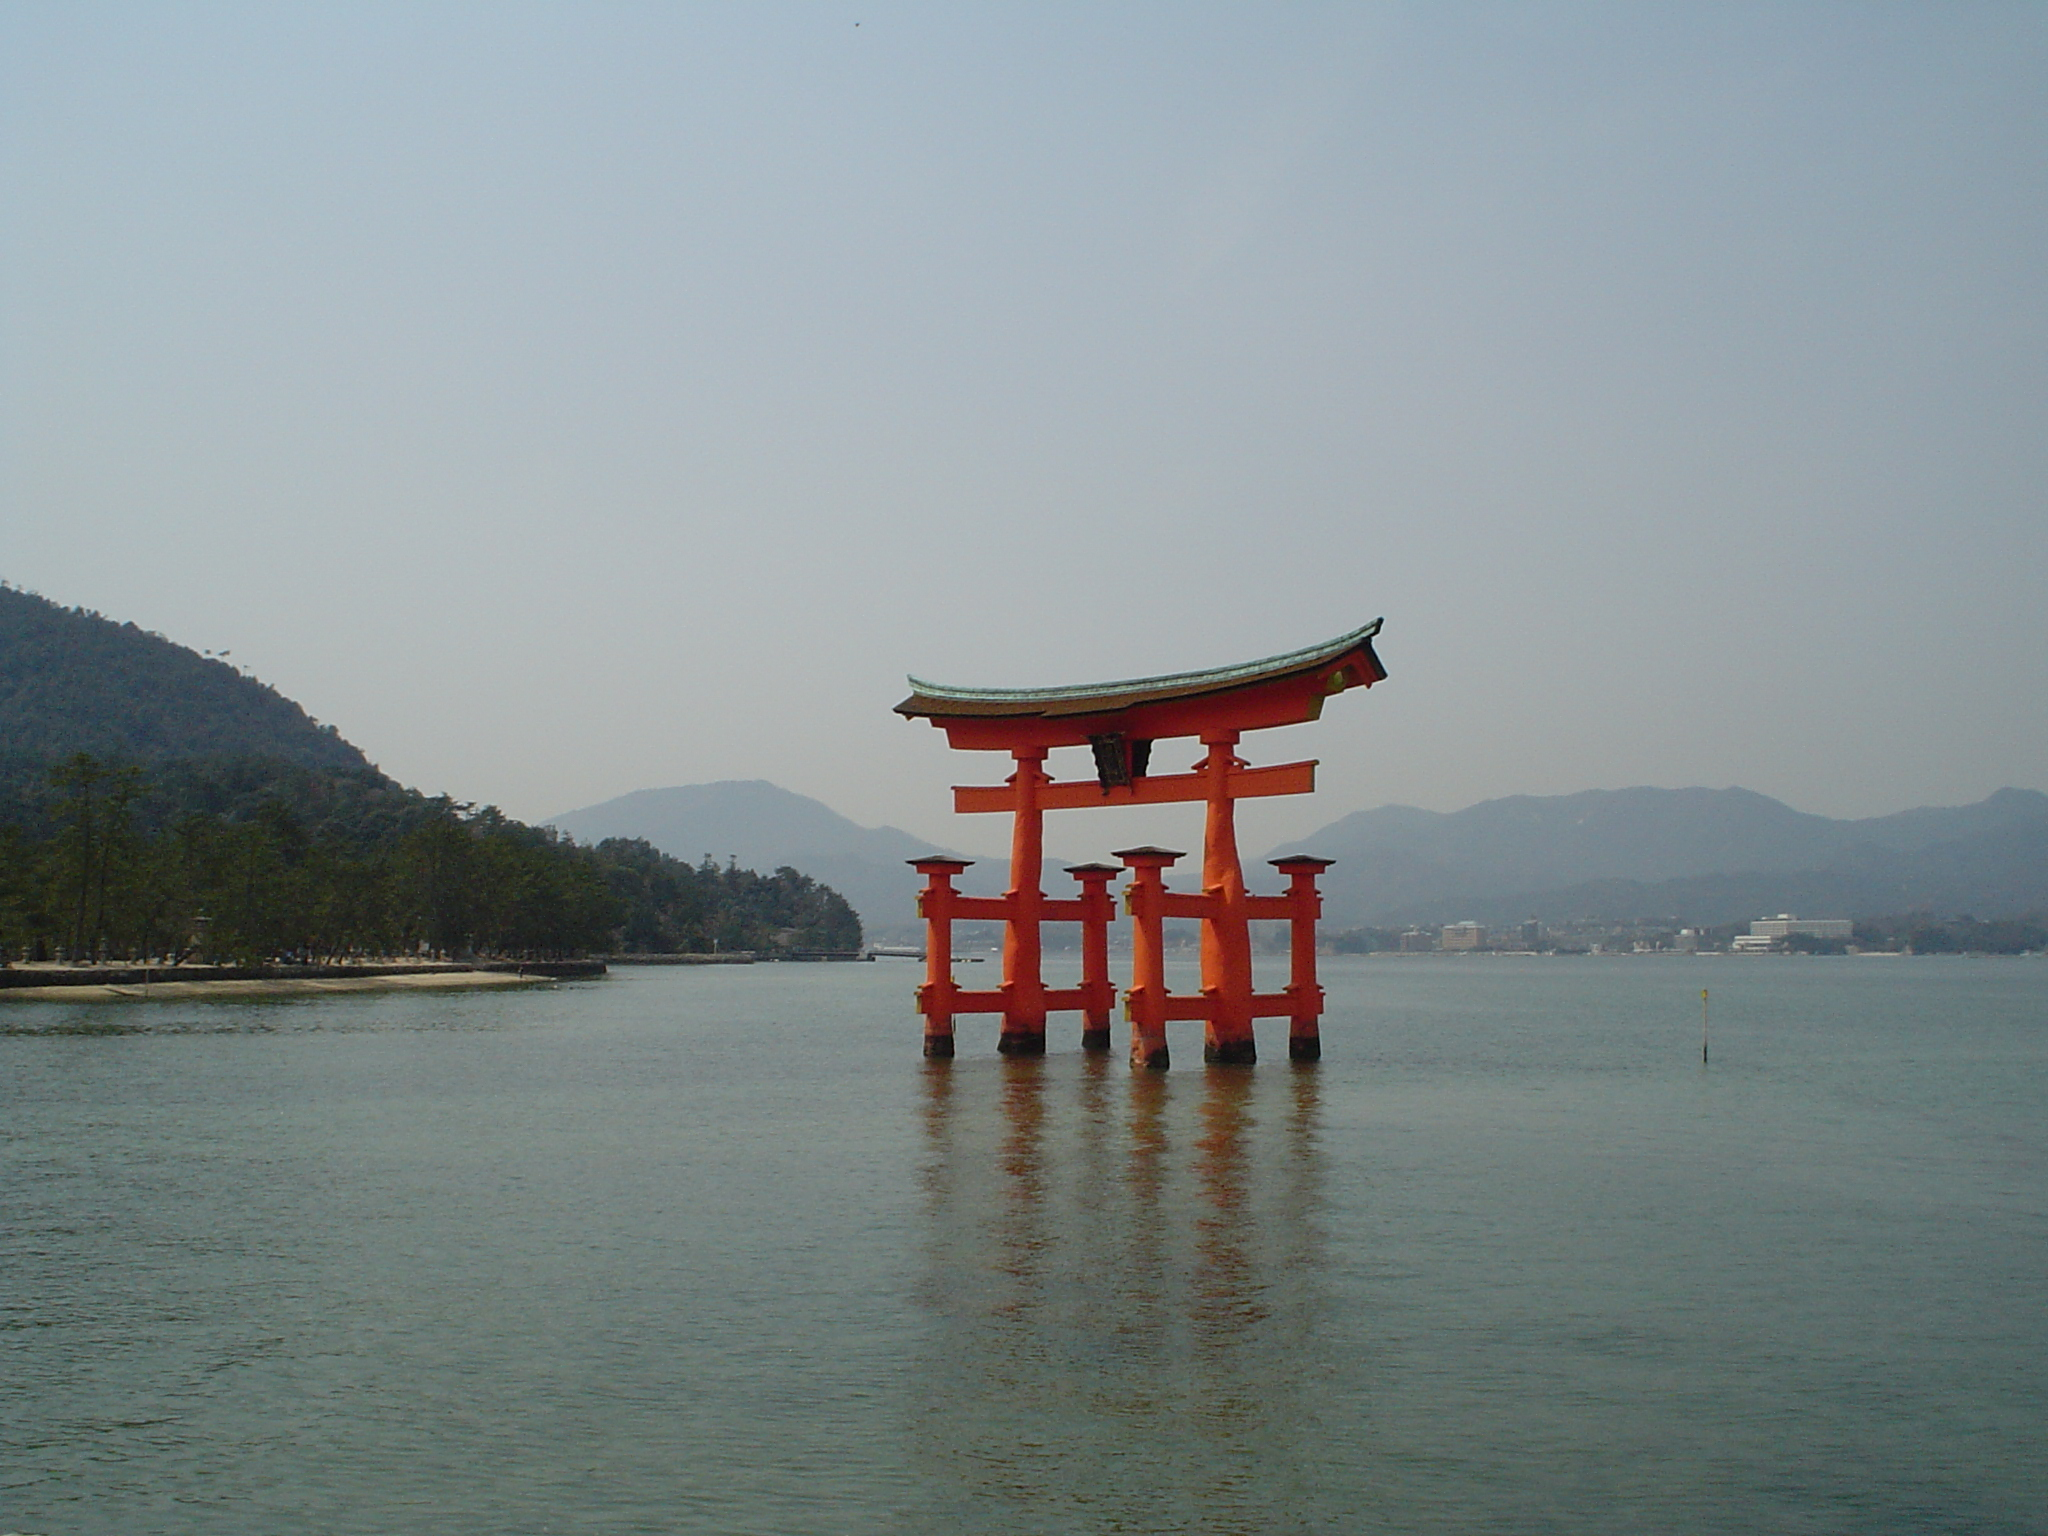
\includegraphics[height=\paperheight]{pics/japan_beach.jpg}
            };
\end{tikzpicture}

\end{frame}

%%%%%%%%%%%%%%%%%%%%%%%%%%%%%%%%%%%%%%%%%%%%%%%%%%
\begin{frame}[fragile]{}

 \begin{tikzpicture}
 % x (kleiner = weiter nach links) y (kleiner = weiter nach unten)
             \put (-15,-157.3) 
{ 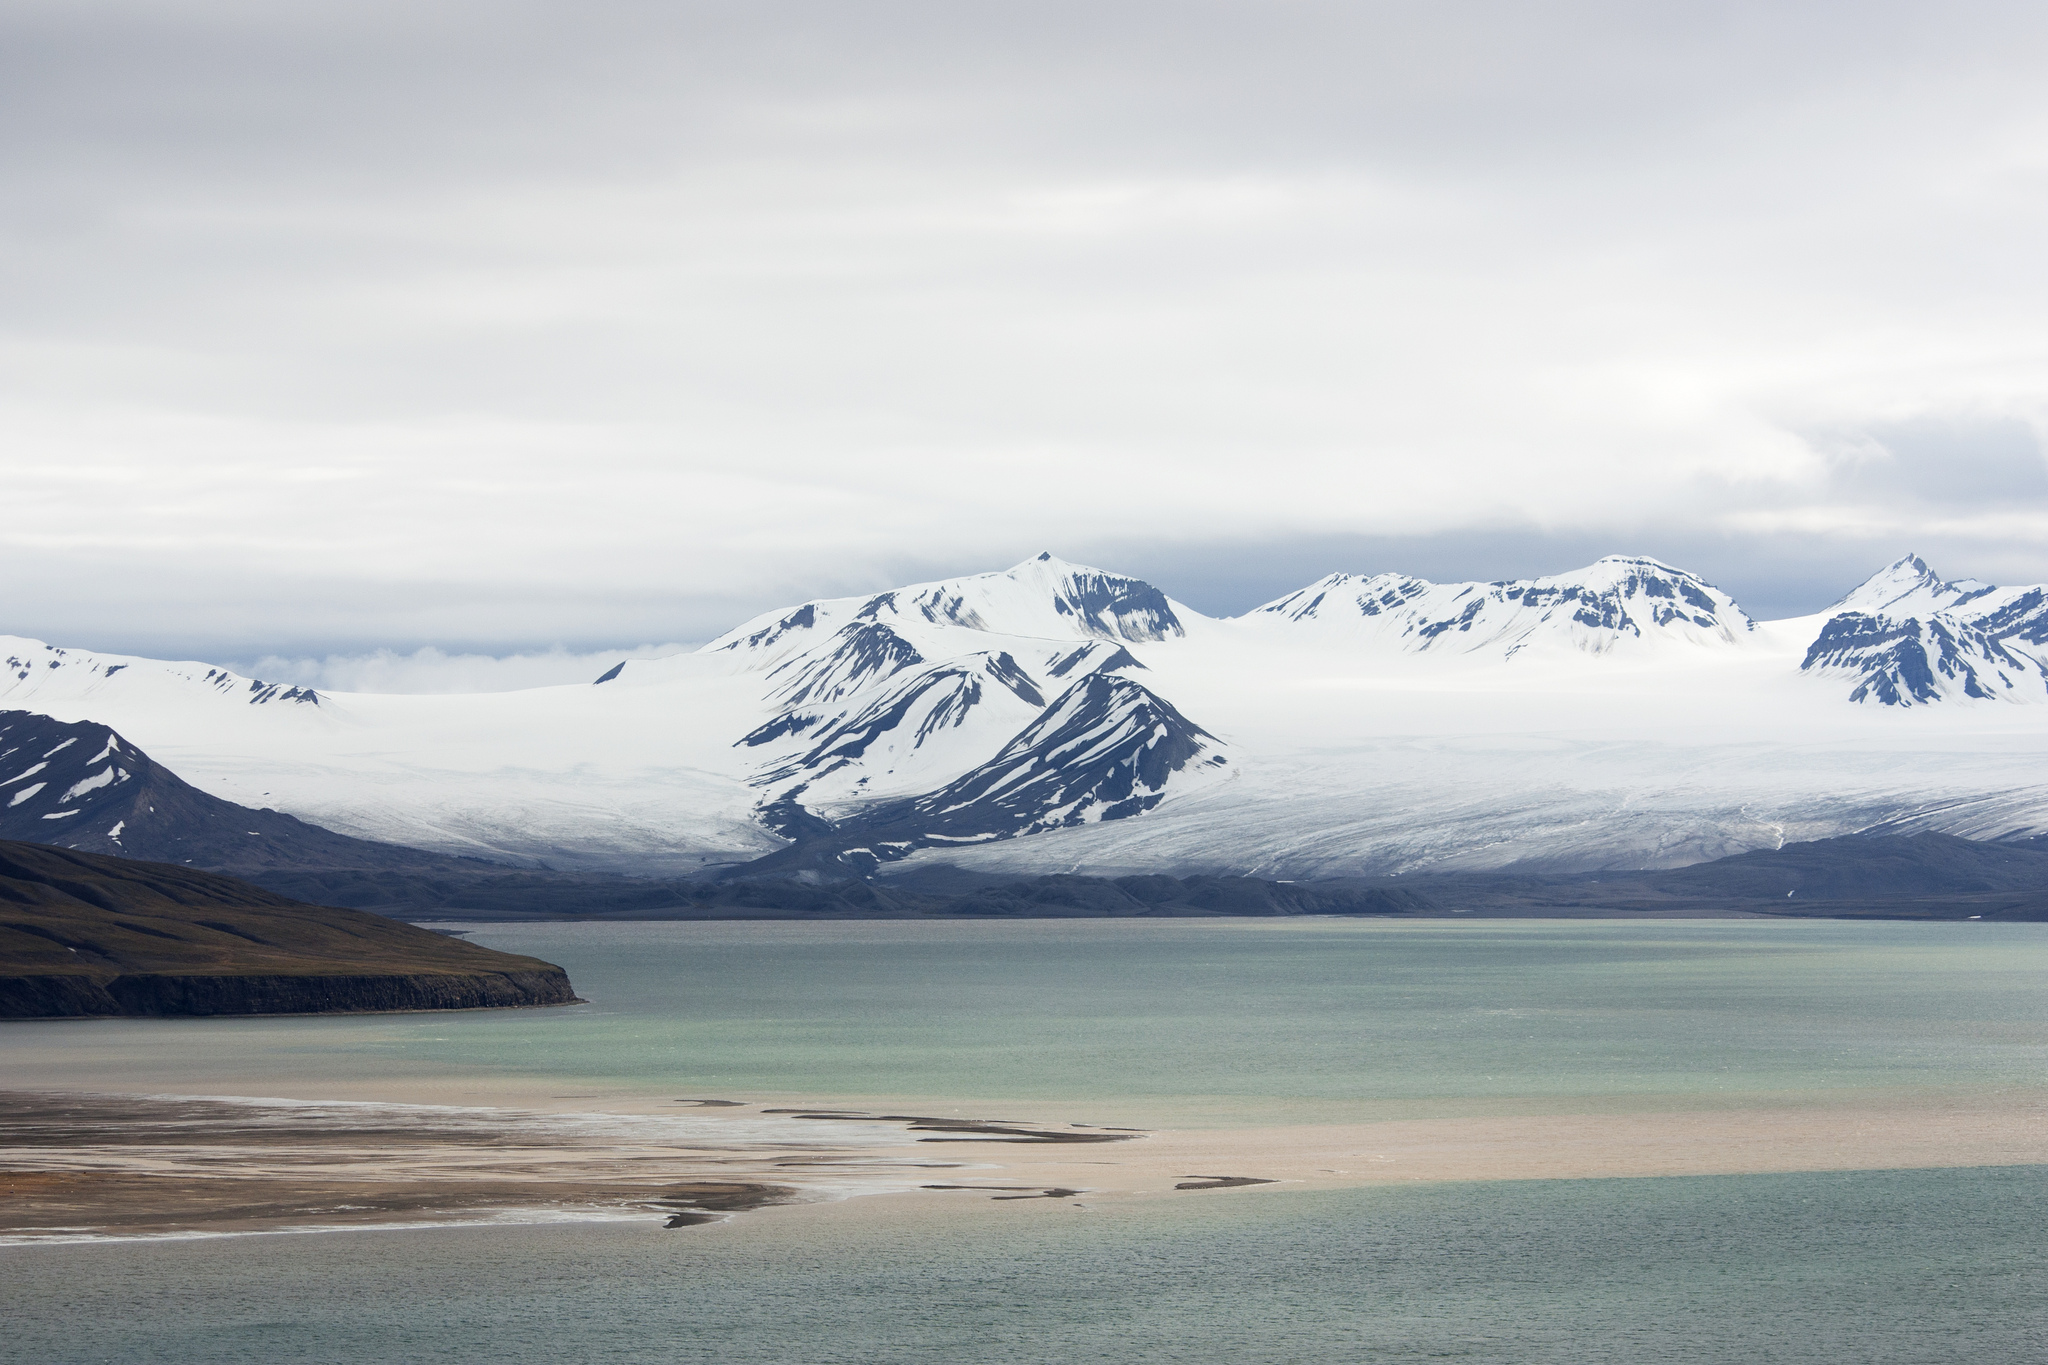
\includegraphics[height=\paperheight]{pics/ice_beach.jpg}
            };
\end{tikzpicture}

\end{frame}

%%%%%%%%%%%%%%%%%%%%%%%%%%%%%%%%%%%%%%%%%%%%%%%%%%
\begin{frame}[fragile]{}

 \begin{tikzpicture}
 % x (kleiner = weiter nach links) y (kleiner = weiter nach unten)
             \put (-23,-157.3) 
{ 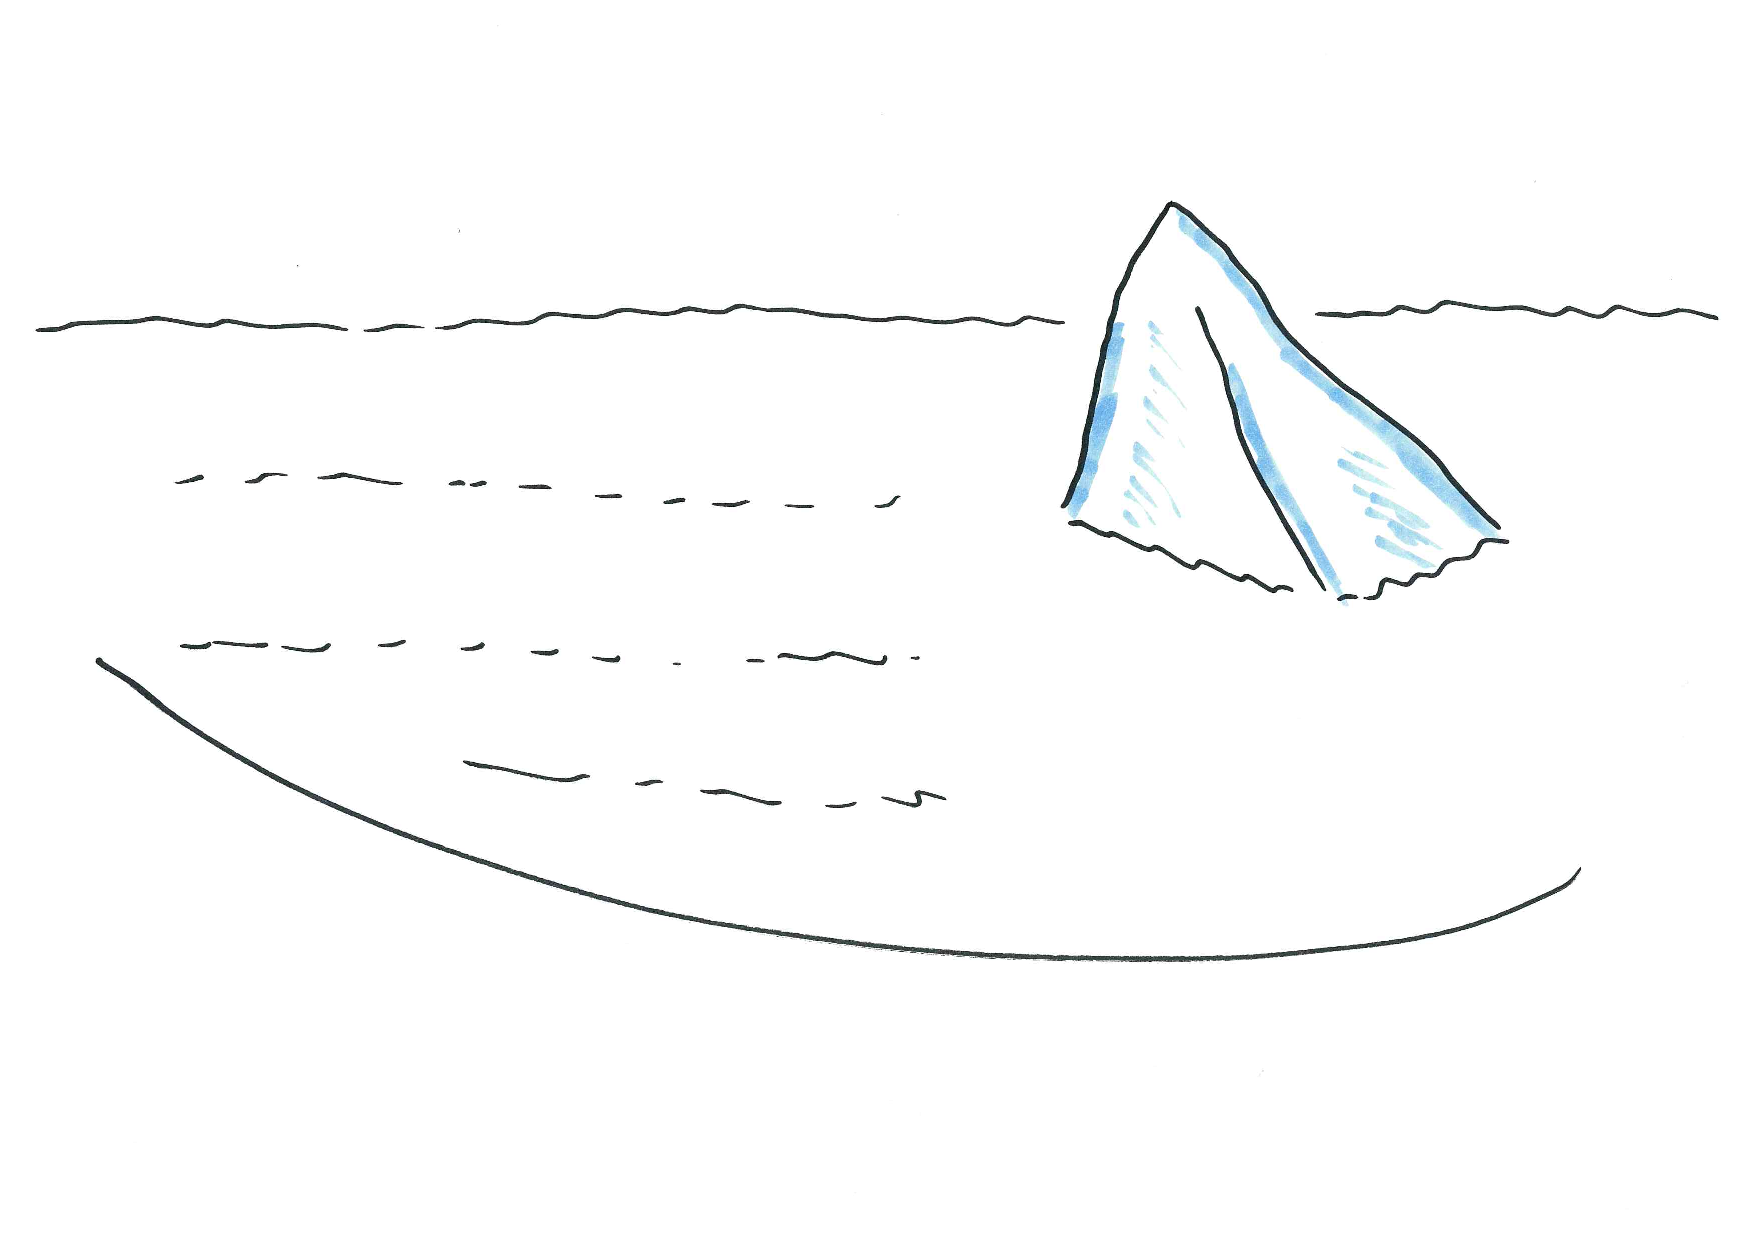
\includegraphics[height=\paperheight]{pics/eine_skizze_meines_urlaubs.pdf}
            };
\end{tikzpicture}

\end{frame}

%-----------------------------------------------------------------------------------------------------------------------------------
\numberednote{

\begin{itemize}
\item wenn ich eine skizze meines urlaubs male, dann gibt es euch vielleicht eine chance, Rückfragen zu stellen und dinge zu klären

\item was ist das da für ein felsen im wasser, und wieso ist der blau? -> Das ist kein Felsen, sondern ein Eisberg.

\item Offensichtliches bleibt gern unerwähnt.
\end{itemize}
}

%%%%%%%%%%%%%%%%%%%%%%%%%%%%%%%%%%%%%%%%%%%%%%%%%%
\begin{frame}[fragile]{\de{WARNUNG}\en{WARNING}}

\begin{center}
{
\LARGE
\de{Hier bei uns passiert gerade dasselbe!}\en{Here the same happens!}
}
\end{center}

\end{frame}

%-----------------------------------------------------------------------------------------------------------------------------------
\numberednote{

Vieles, was ich sage, versteht Ihr vermutlich anders als ich es erwarte
}

%%%%%%%%%%%%%%%%%%%%%%%%%%%%%%%%%%%%%%%%%%%%%%%%%%
\begin{frame}[fragile]{}

\begin{center}
{
\LARGE
WORKSHOP}
\end{center}

\end{frame}


%%%%%%%%%%%%%%%%%%%%%%%%%%%%%%%%%%%%%%%%%%%%%%%%%%
\begin{frame}[fragile]{\de{Unsere Domäne}\en{Our Domain}: eCommerce}

\onslide+<2->
 \begin{tikzpicture}
 % x (kleiner = weiter nach links) y (kleiner = weiter nach unten)
            \put (-10,-20) { 
\includegraphics[width=.4\textwidth]{pics/onlineshopping.png} };
\end{tikzpicture}

\onslide+<3->
 \begin{tikzpicture}
            \put (90,-120) { 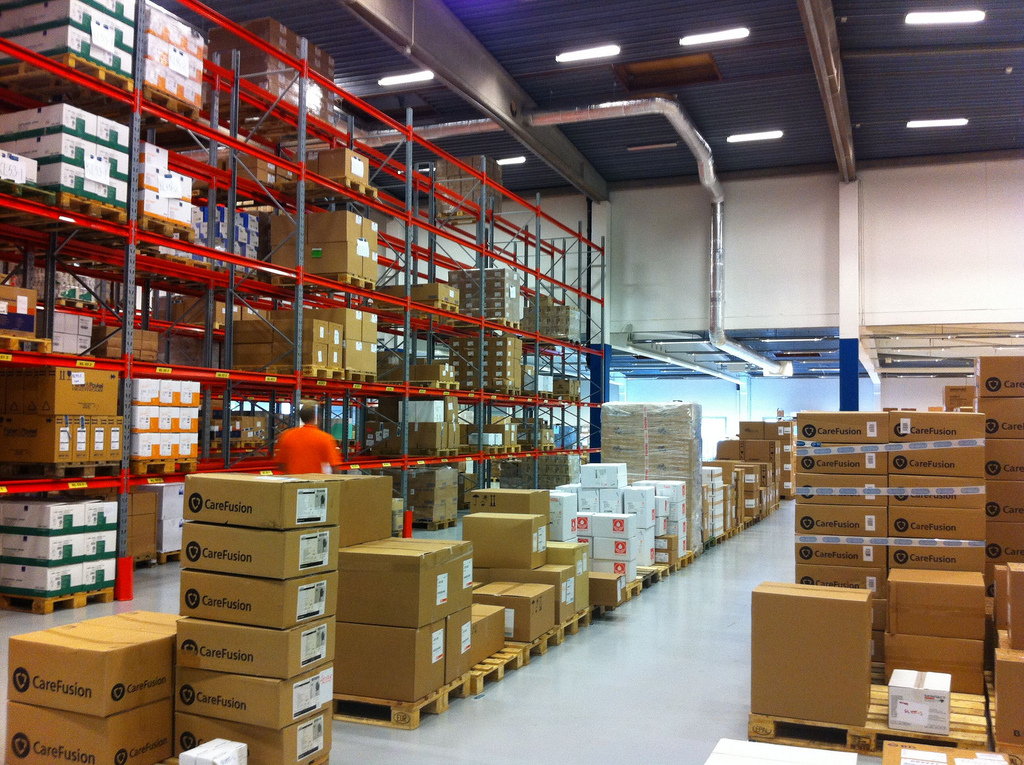
\includegraphics[height=.4\textheight]{pics/warehouse.jpg} };
\end{tikzpicture}

\onslide+<4->
 \begin{tikzpicture}
            \put (180,30) { 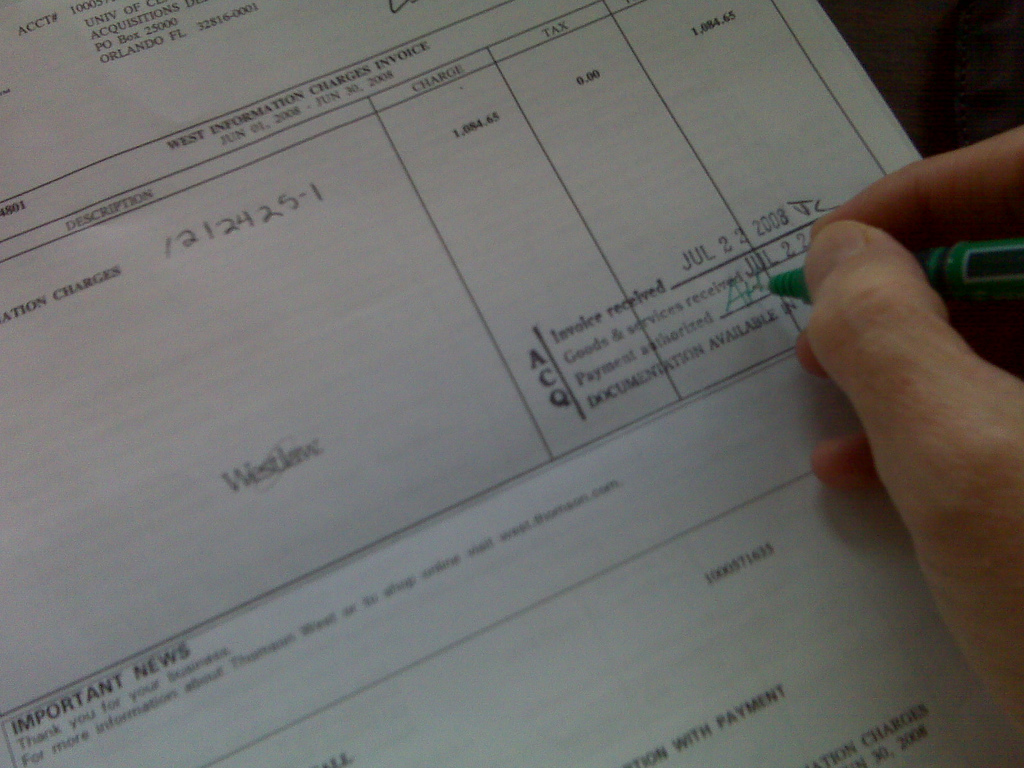
\includegraphics[width=.4\textwidth]{pics/ordering.jpg} };
\end{tikzpicture}

\end{frame}

%-----------------------------------------------------------------------------------------------------------------------------------
\numberednote{

\begin{itemize}
\item Onlineshop
\item Lagerhaltung
\item Bestellungen
\end{itemize}
}

%%%%%%%%%%%%%%%%%%%%%%%%%%%%%%%%%%%%%%%%%%%%%%%%%%
%%%%%%%%%%%%%%%%%%%%%%%%%%%%%%%%%%%%%%%%%%%%%%%%%%
\begin{frame}[fragile]{EventStorming I}

\de{Capture} \textbf{Events} \de{erfassen}

\begin{itemize}
\item \de{Ereignis in der Vergangenheit}\en{Something that happened in the past}
\item \de{Relevant für den Fachbereich}\en{Relevant for the business}
\item \de{Beobachtbar im System}\en{Observable in the system}
\end{itemize}

\begin{itemize}
\item \de{Beschrieben durch \textbf{Verb in der Vergangenheit}}\en{Described by a \textbf{verb in the past}}
\end{itemize}

\end{frame}

%%%%%%%%%%%%%%%%%%%%%%%%%%%%%%%%%%%%%%%%%%%%%%%%%%
\begin{frame}[fragile]{\de{Beispiel}\en{Example}}

\begin{center}

\includegraphics[width=.5\textwidth]{pics/eventstorming1.jpg}
\end{center}

\end{frame}


%-----------------------------------------------------------------------------------------------------------------------------------
\numberednote{

\textbf{Übung:} Events der Domäne erfassen! (20 - 30 min)

~\\
\textbf{Was kann schiefgehen:}

\begin{itemize}
\item kein Verb
\item nicht in der Vergangenheit
\item außerhalb des Beobachtbaren
\begin{itemize}
\item Kunde beginnt sich für unsere Produkte zu interessieren
\item Kunde erhält seine Lieferung
\end{itemize}
\end{itemize}

}


%%%%%%%%%%%%%%%%%%%%%%%%%%%%%%%%%%%%%%%%%%%%%%%%%%
\begin{frame}[fragile]{\de{So kann das aussehen}\en{That's how it can look like}}

\begin{center}
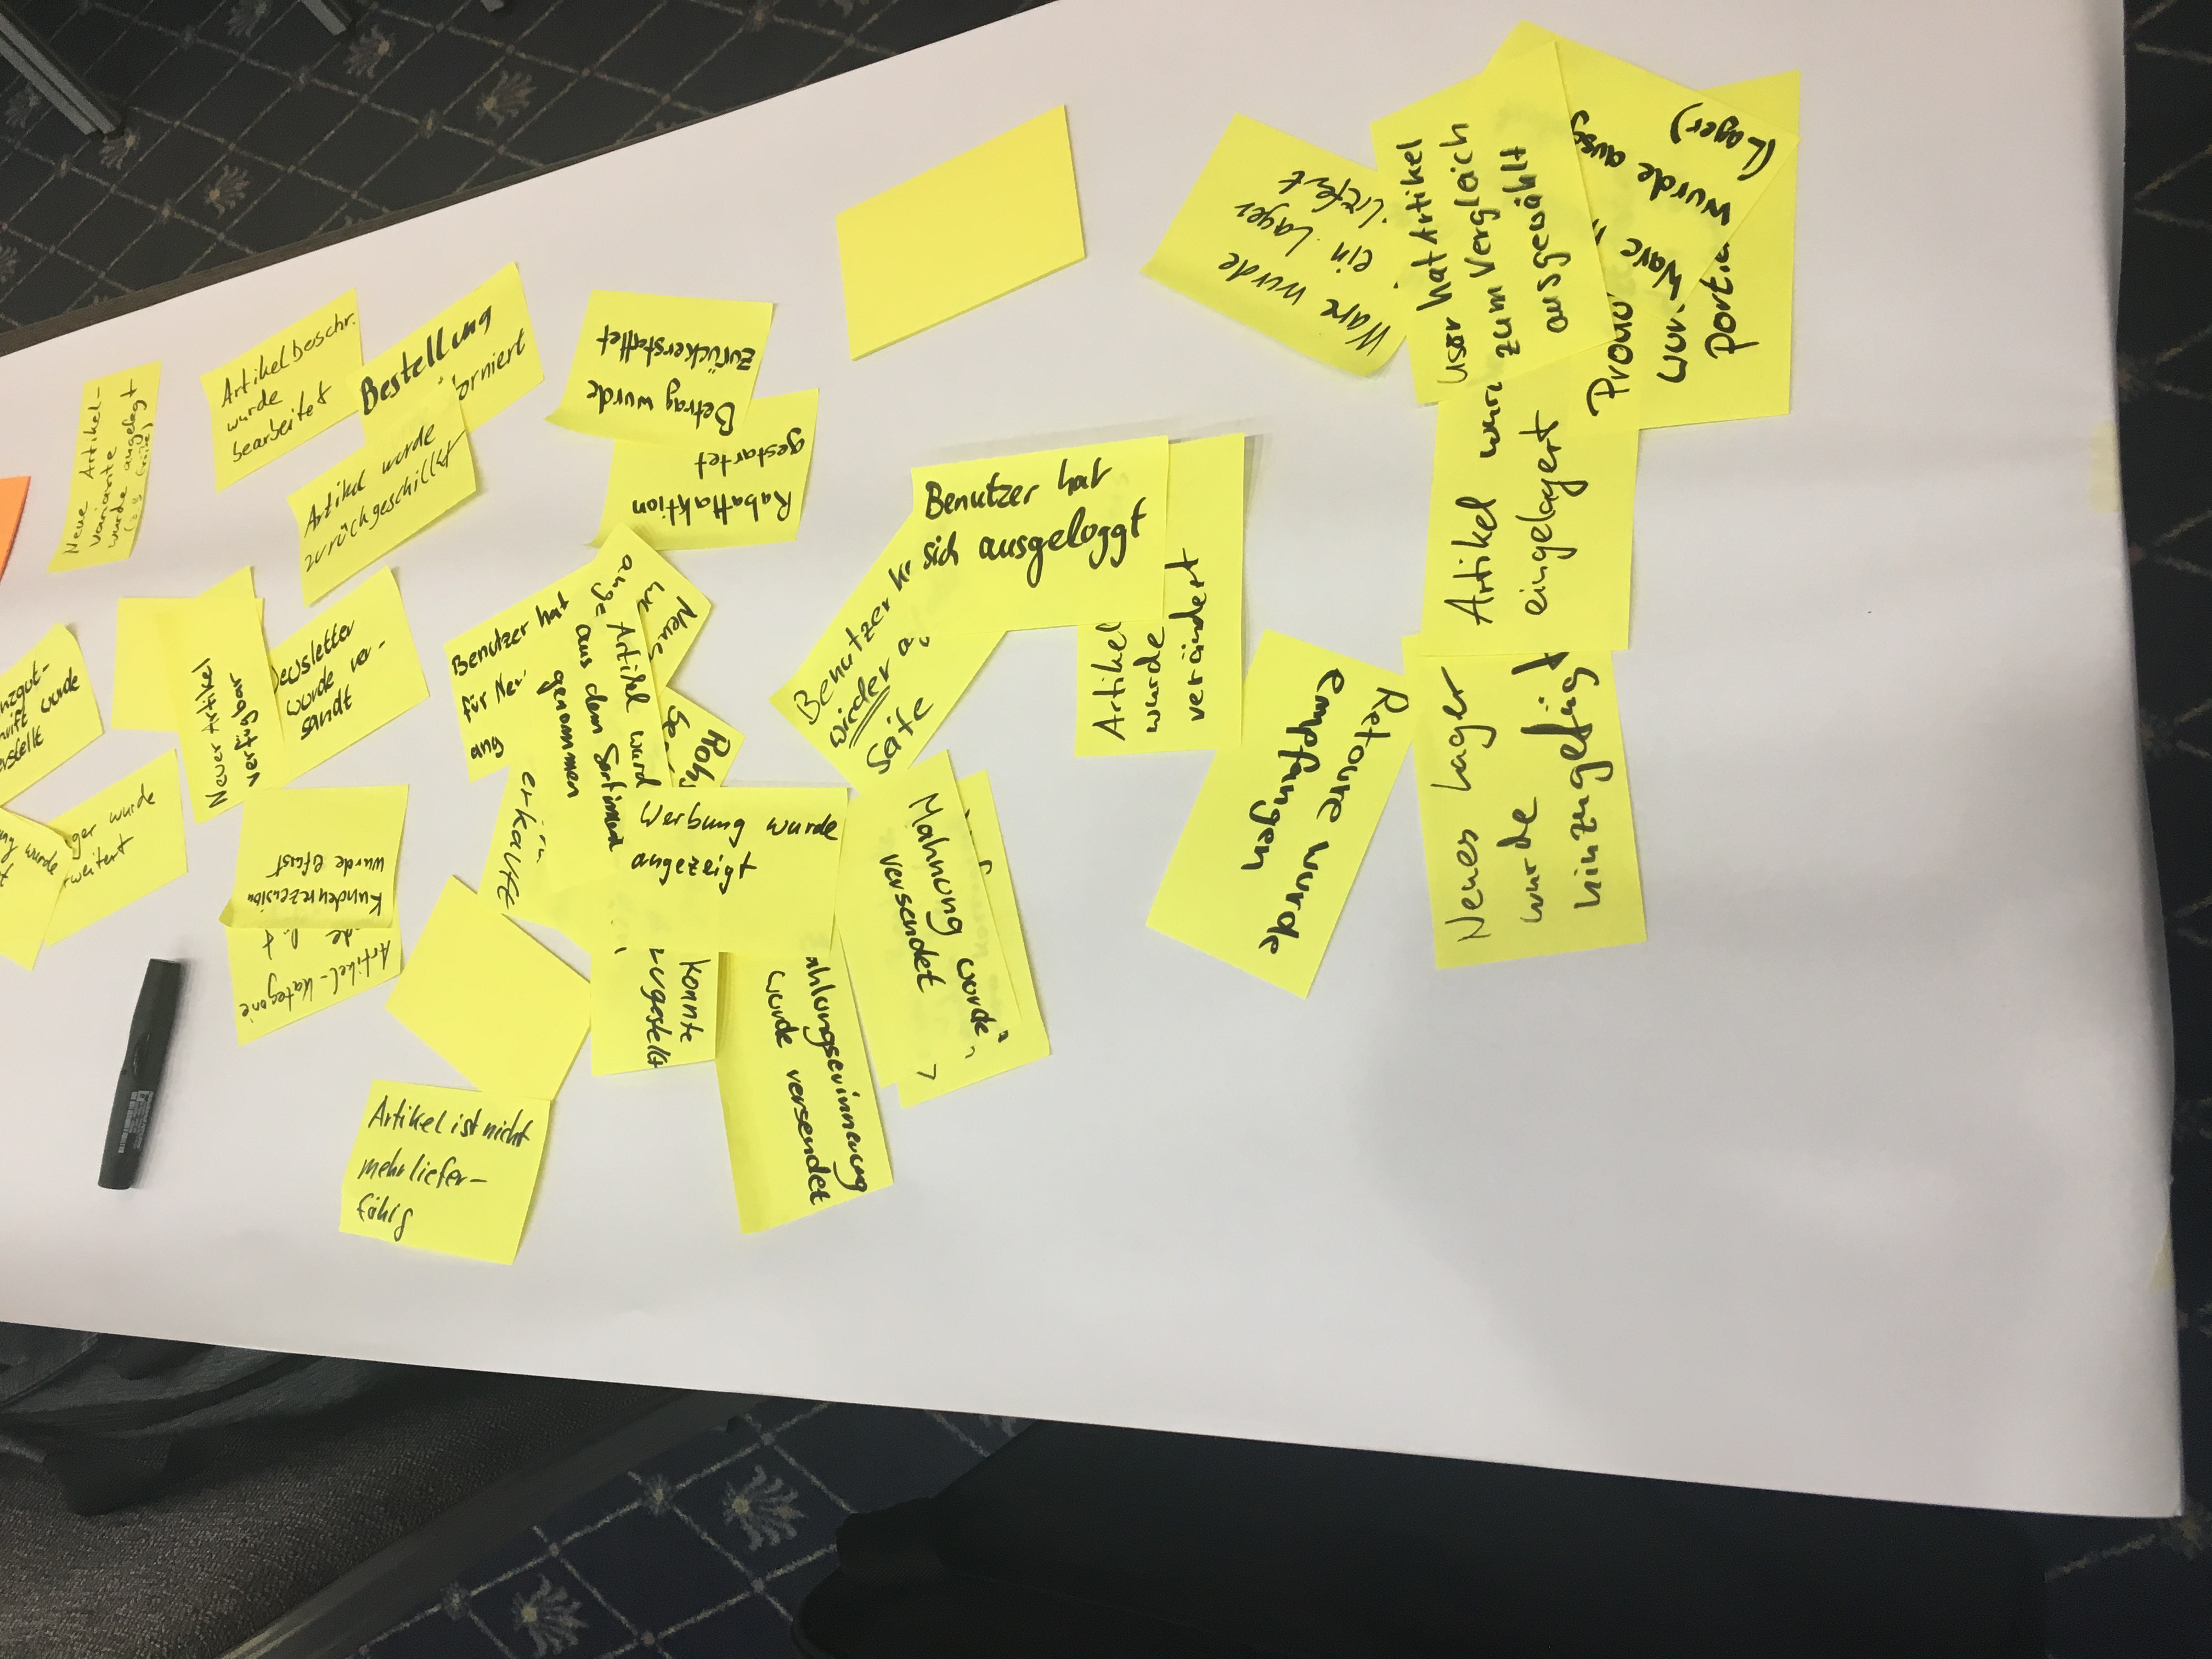
\includegraphics[width=.5\textwidth]{pics/modelling_events.jpg}
\end{center}

\end{frame}


%%%%%%%%%%%%%%%%%%%%%%%%%%%%%%%%%%%%%%%%%%%%%%%%%%
%%%%%%%%%%%%%%%%%%%%%%%%%%%%%%%%%%%%%%%%%%%%%%%%%%
\begin{frame}[fragile]{EventStorming II}

\begin{itemize}
\item \de{Viele Events unterliegen einer zeitlichen Abfolge}\en{Many events are in chronological order}
\item \de{Zeit verläuft \textbf{von links nach rechts}}\en{Time runs \textbf{from left to right}}
\end{itemize}

\end{frame}

%%%%%%%%%%%%%%%%%%%%%%%%%%%%%%%%%%%%%%%%%%%%%%%%%%
\begin{frame}[fragile]{\de{Zeit}\en{Time}}

\begin{center}
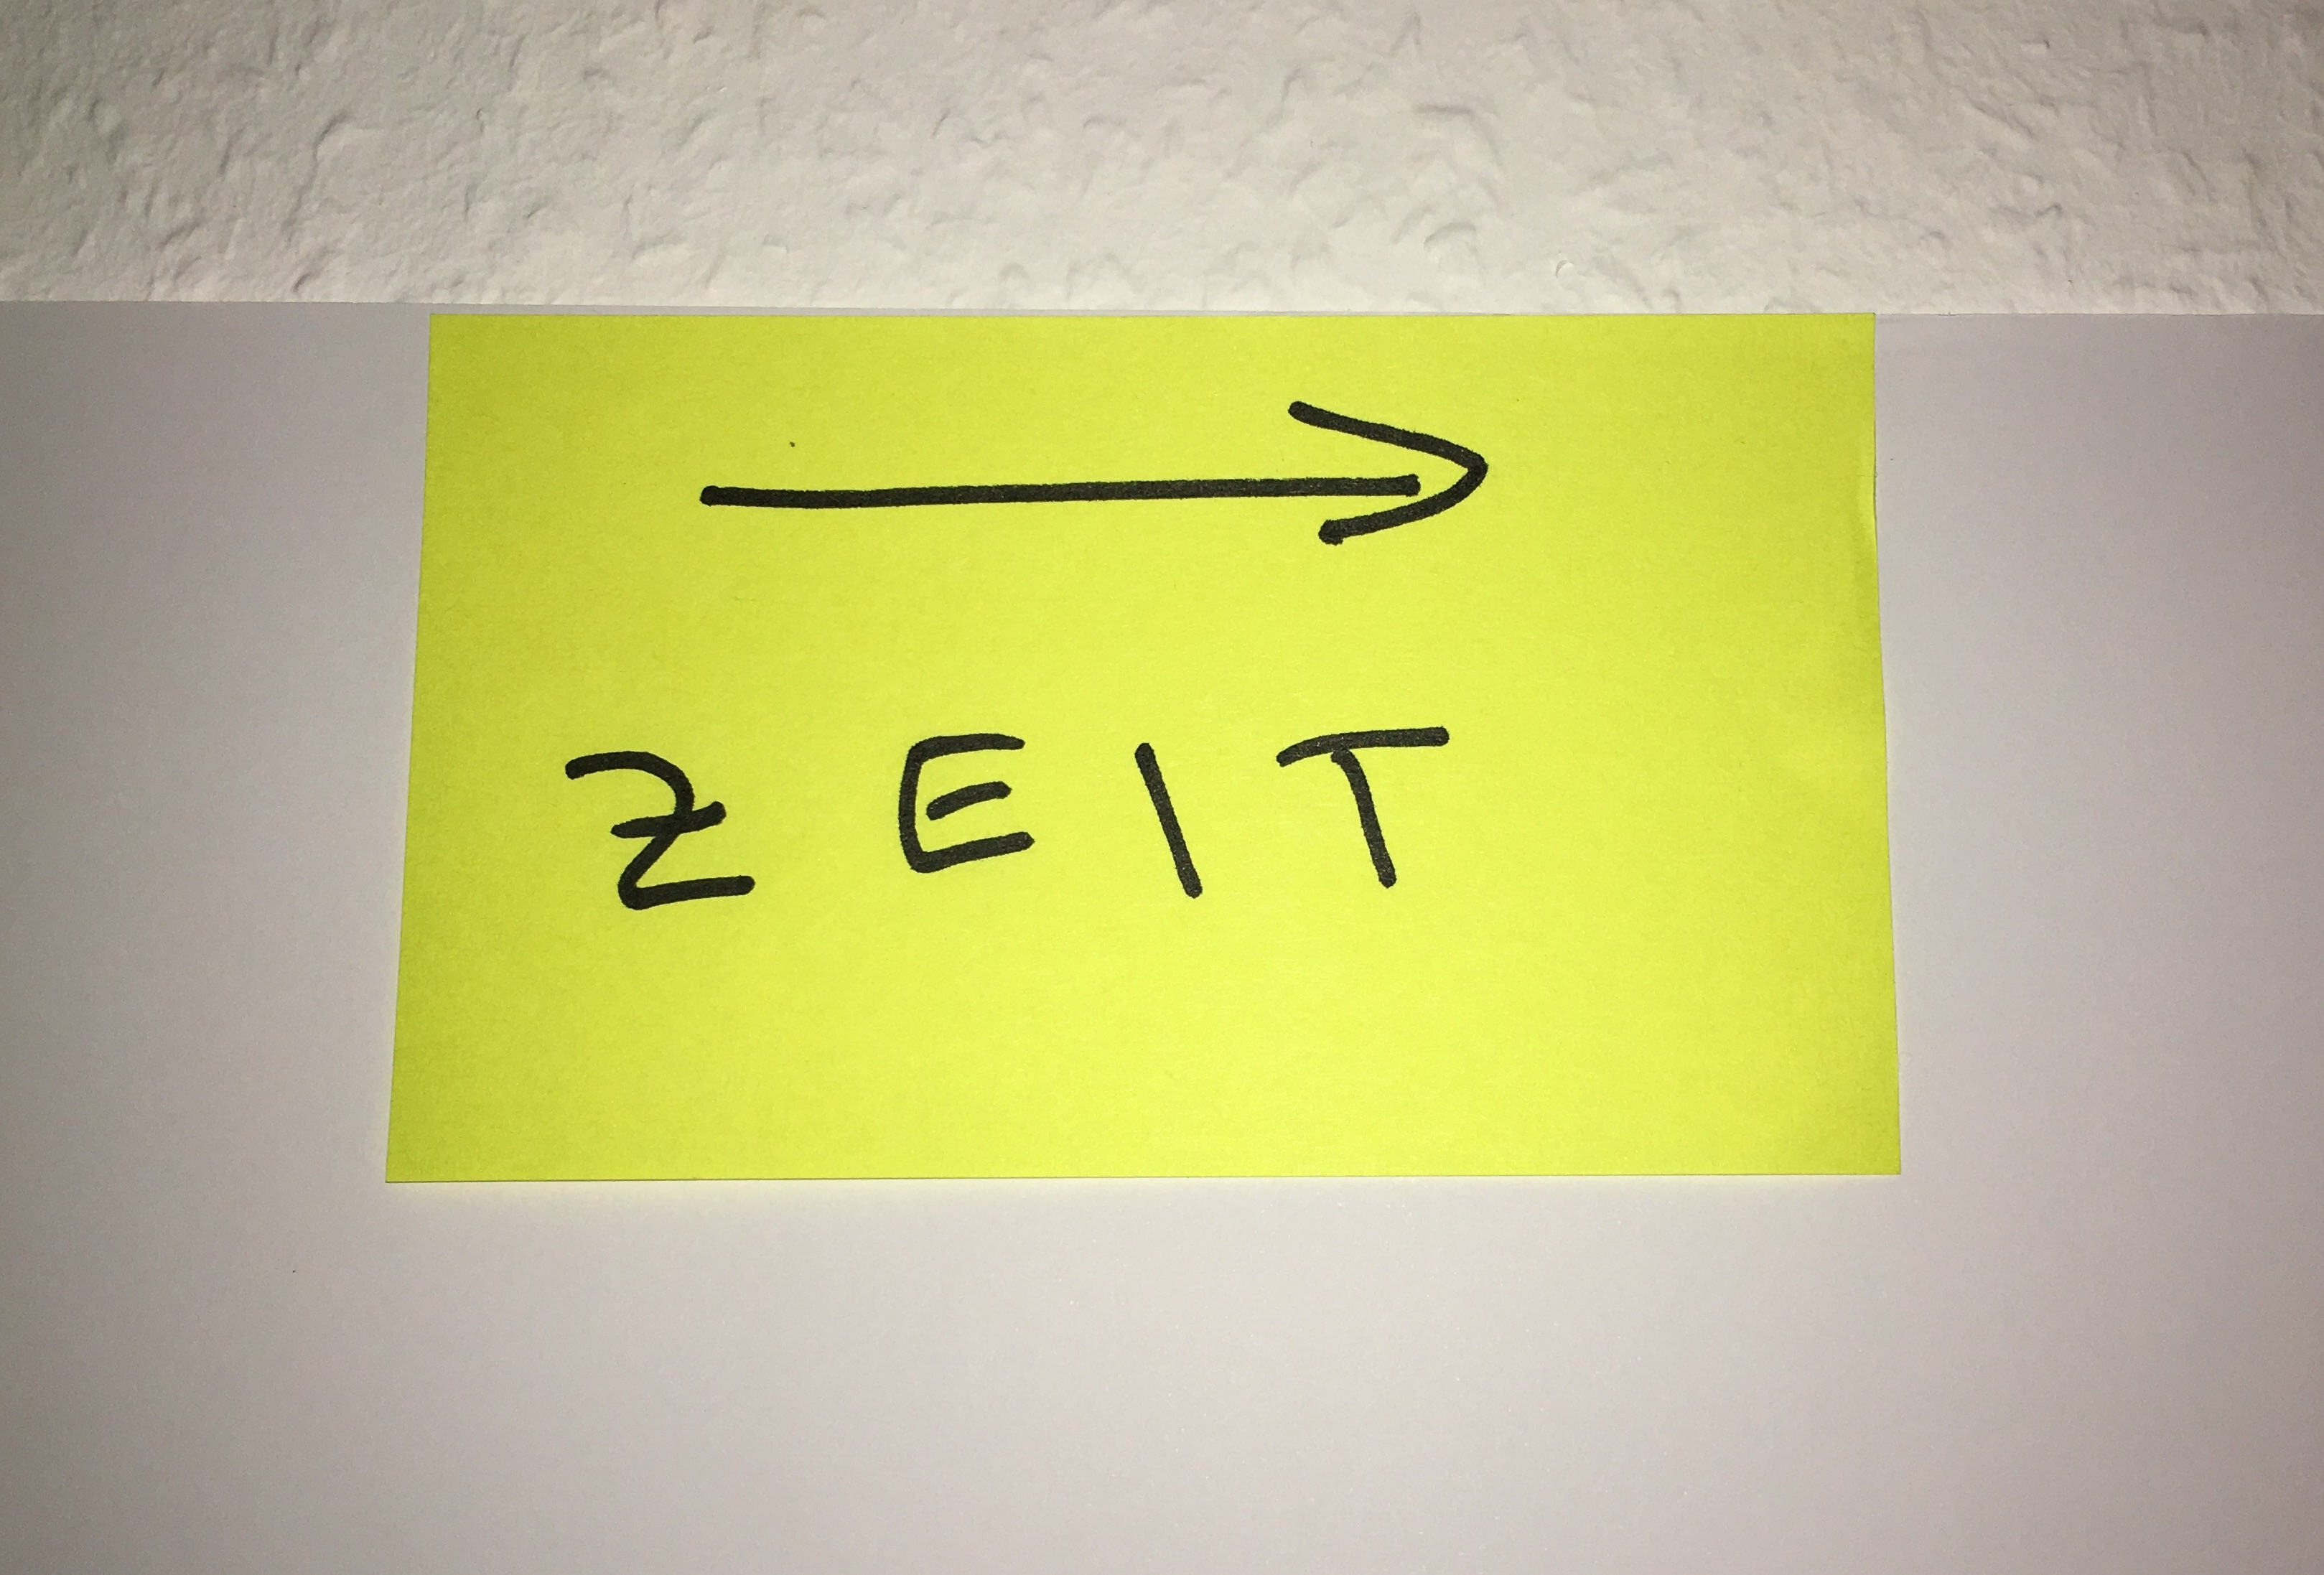
\includegraphics[width=.5\textwidth]{pics/eventstorming_zeit.jpg}
\end{center}

\end{frame}


%%%%%%%%%%%%%%%%%%%%%%%%%%%%%%%%%%%%%%%%%%%%%%%%%%
\begin{frame}[fragile]{\de{Beispiel}\en{Example}}

\begin{center}
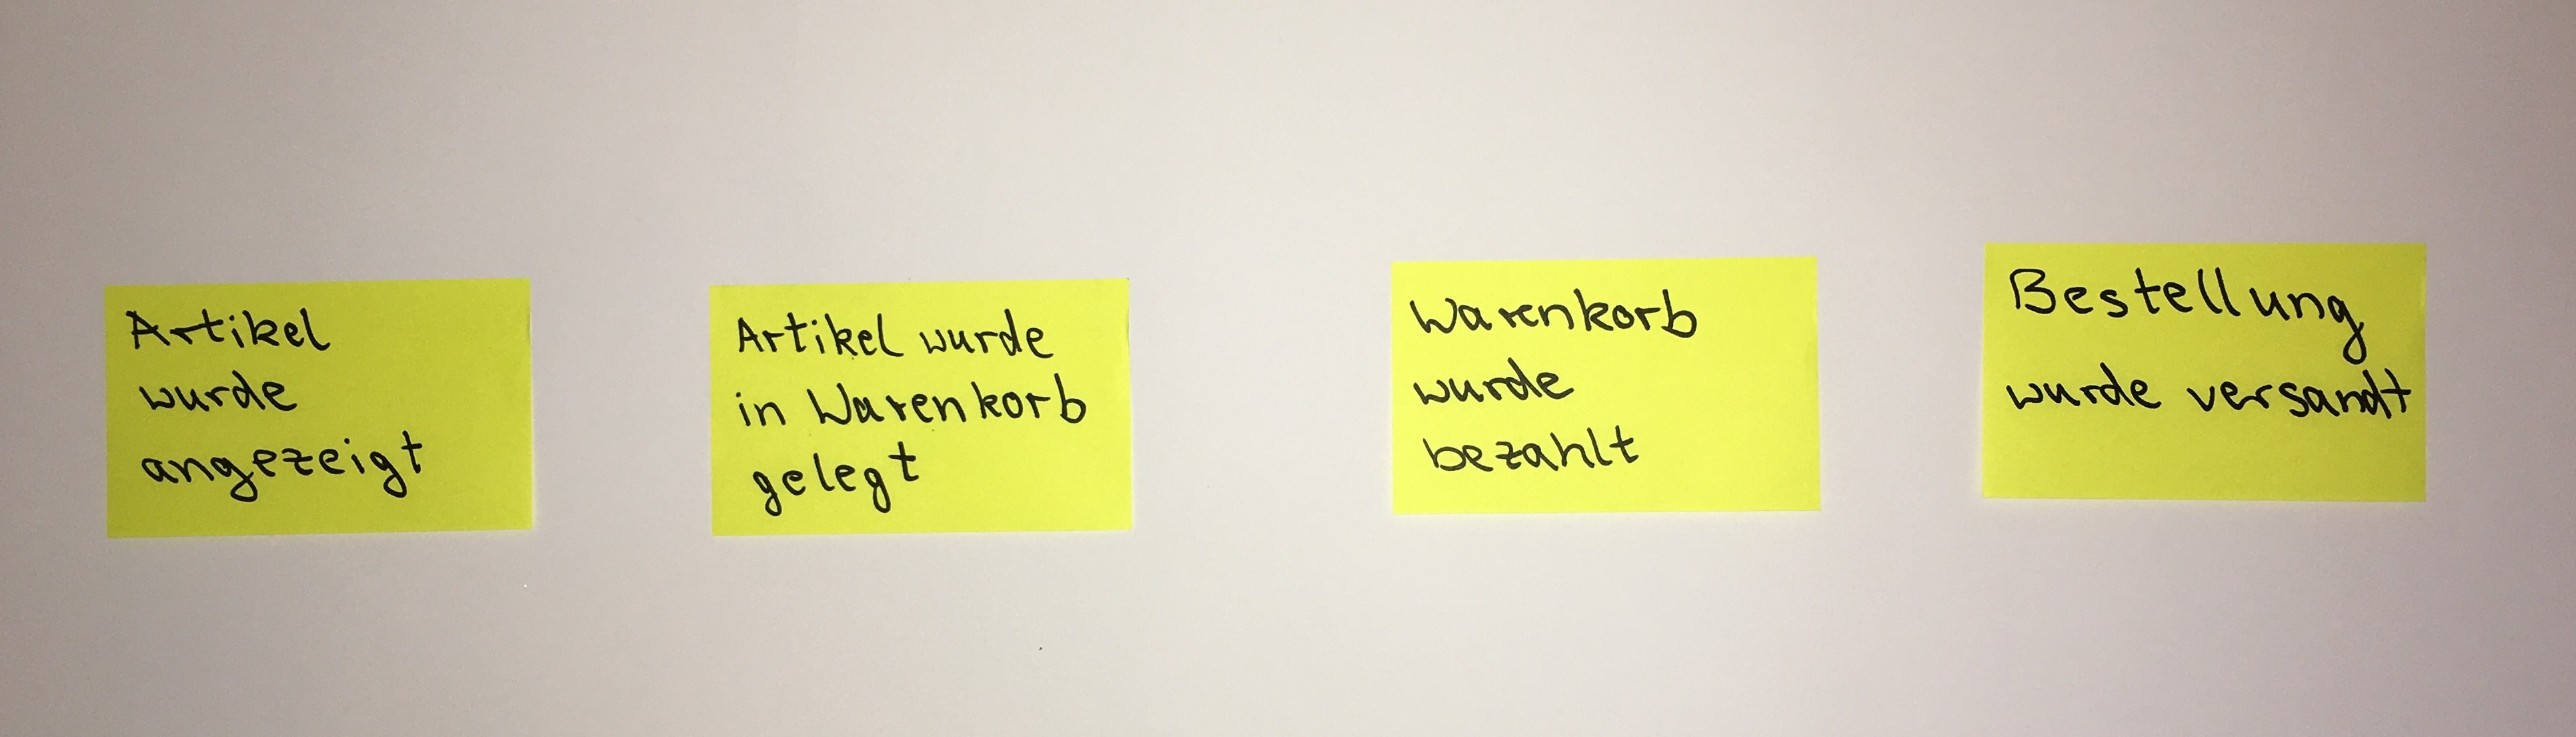
\includegraphics[width=.9\textwidth]{pics/eventstorming_zeitlich_geordnet.jpg}
\end{center}

\end{frame}

%-----------------------------------------------------------------------------------------------------------------------------------
\numberednote{

\textbf{Übung:}

\begin{itemize}

\item Events in zeitliche Reihenfolge bringen

\item Redundanzen entfernen

\item Fehlendes ergänzen

\item Ubiquitous Language erfassen

\item Begriffe schärfen und vereinheitlichen

\end{itemize}

~\\
\textbf{Kritische Fragen:}
\begin{itemize}
\item Was wenn dies vor jenem passiert?
\end{itemize}

~\\
\textbf{Was kann schiefgehen?}

\begin{itemize}
\item x
\end{itemize}

}

%%%%%%%%%%%%%%%%%%%%%%%%%%%%%%%%%%%%%%%%%%%%%%%%%%
\begin{frame}[fragile]{\de{So kann das aussehen}\en{That's what it can look like}}

\begin{center}
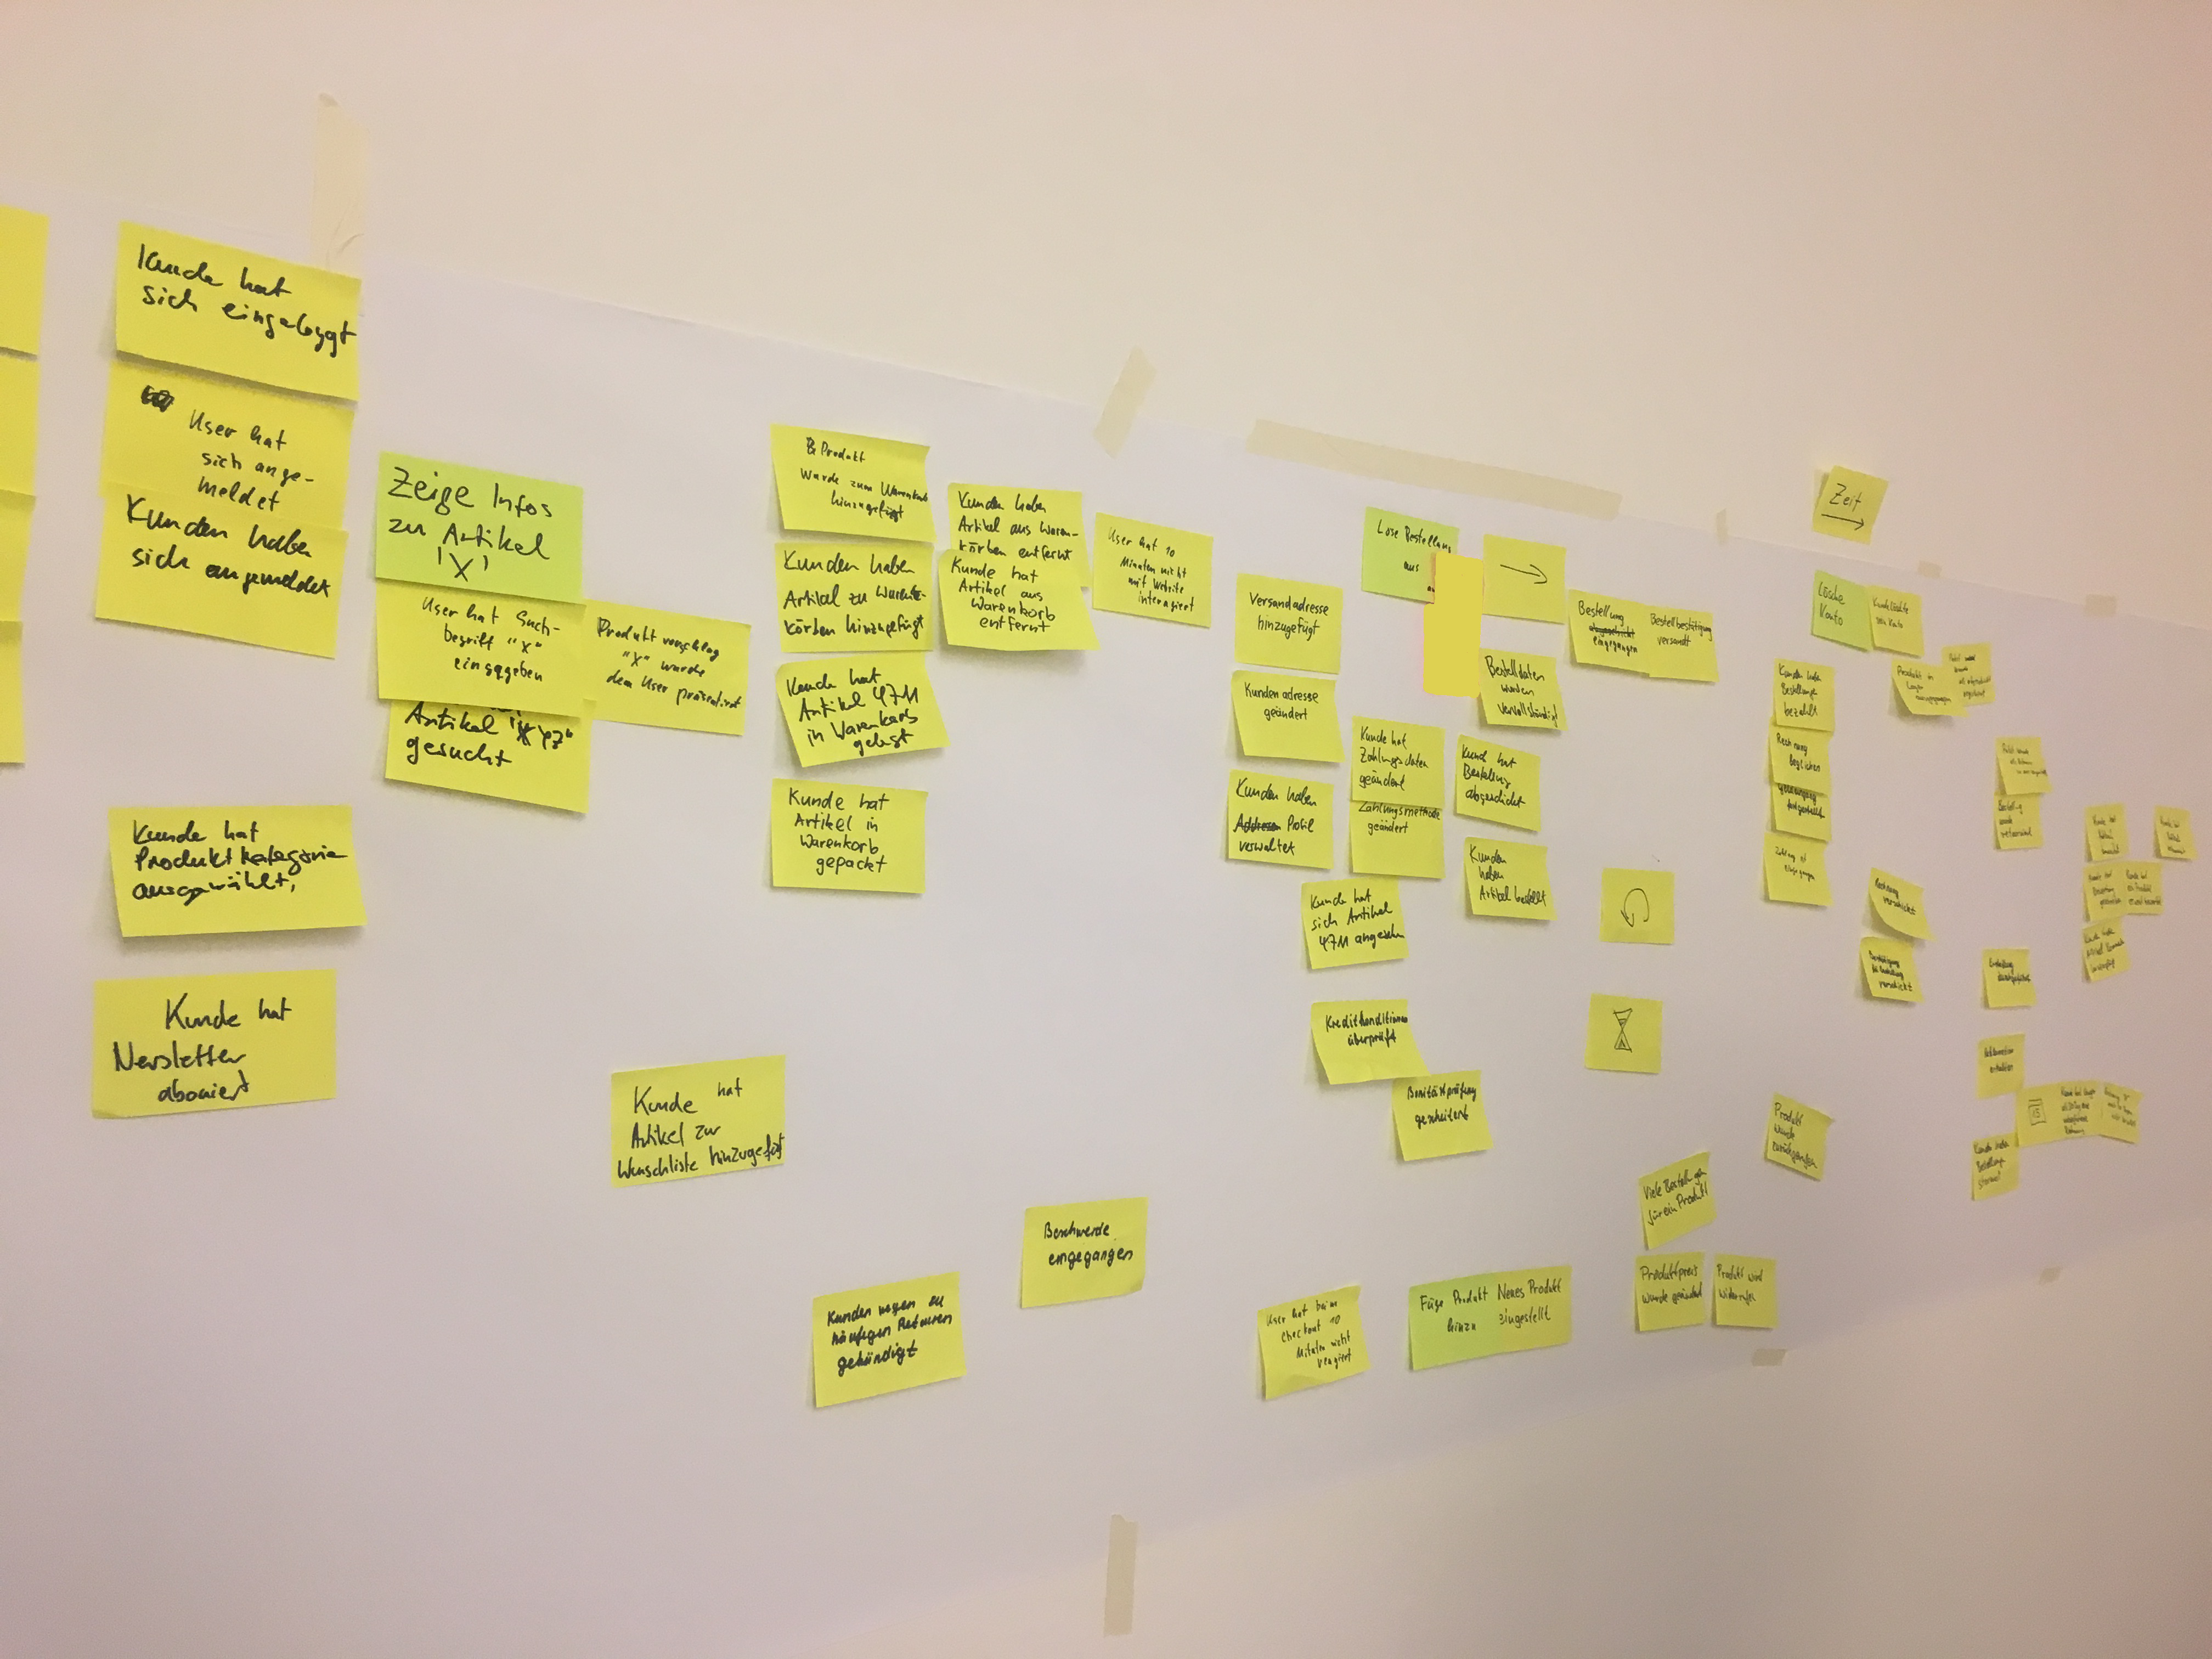
\includegraphics[width=.5\textwidth]{pics/modelling_events_zeit2.jpg}
\end{center}

\end{frame}



%%%%%%%%%%%%%%%%%%%%%%%%%%%%%%%%%%%%%%%%%%%%%%%%%%
\begin{frame}[fragile]{EventStorming III}

\begin{itemize}
\item \de{Vor einem Event muss etwas im System passiert sein:}\en{Each event must be raised by some activity in the system}
\item \textbf{Command}
\item \de{Werden in Befehlsform ausgedrückt}\en{Are expressed in the imperative}
\end{itemize}

\end{frame}

%%%%%%%%%%%%%%%%%%%%%%%%%%%%%%%%%%%%%%%%%%%%%%%%%%
\begin{frame}[fragile]{\de{Beispiel}\en{Example}}

\begin{center}
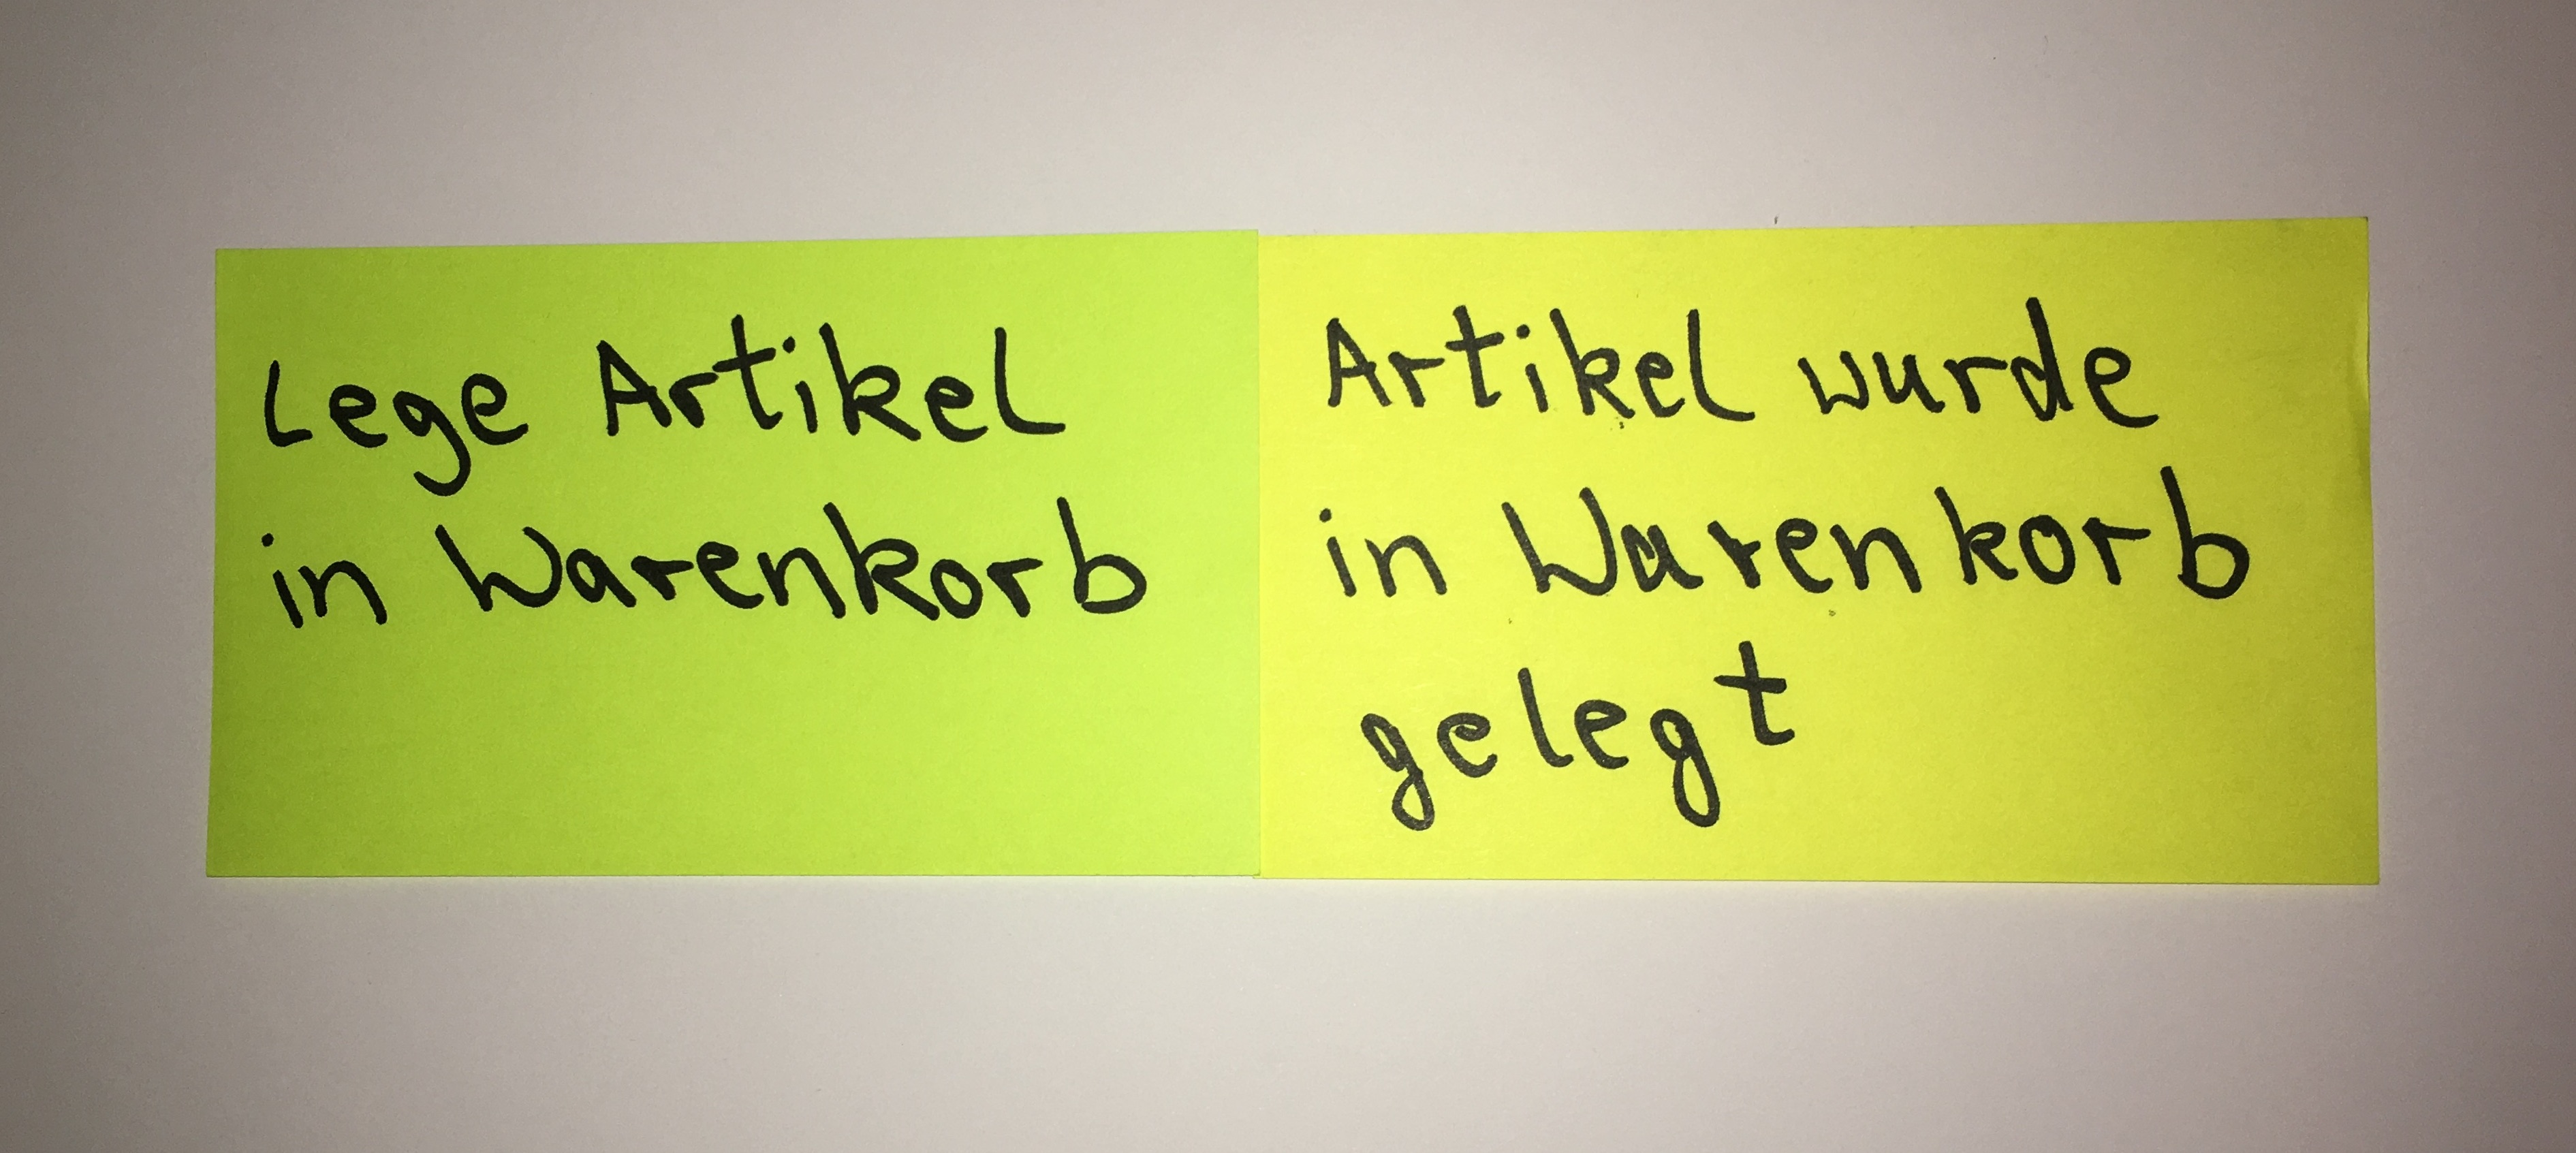
\includegraphics[width=.7\textwidth]{pics/eventstorming2.jpg}
\end{center}

\end{frame}


%%%%%%%%%%%%%%%%%%%%%%%%%%%%%%%%%%%%%%%%%%%%%%%%%%
\begin{frame}[fragile]{EventStorming III}

\begin{itemize}
\item \de{Nicht alle Commands führen direkt zu einem Event}\en{Not all commands lead to an event unconditionally}
\item \textbf{Constraints} \de{müssen berücksichtigt werden}\en{need to be considered}
\item \de{Entscheidung als Frage formulieren}\en{Decision is formulated as question}
\item \de{Events beantworten die Frage}\en{Events answer the question}
\end{itemize}

\end{frame}

%%%%%%%%%%%%%%%%%%%%%%%%%%%%%%%%%%%%%%%%%%%%%%%%%%
\begin{frame}[fragile]{\de{Beispiel}\en{Example}}

\begin{center}
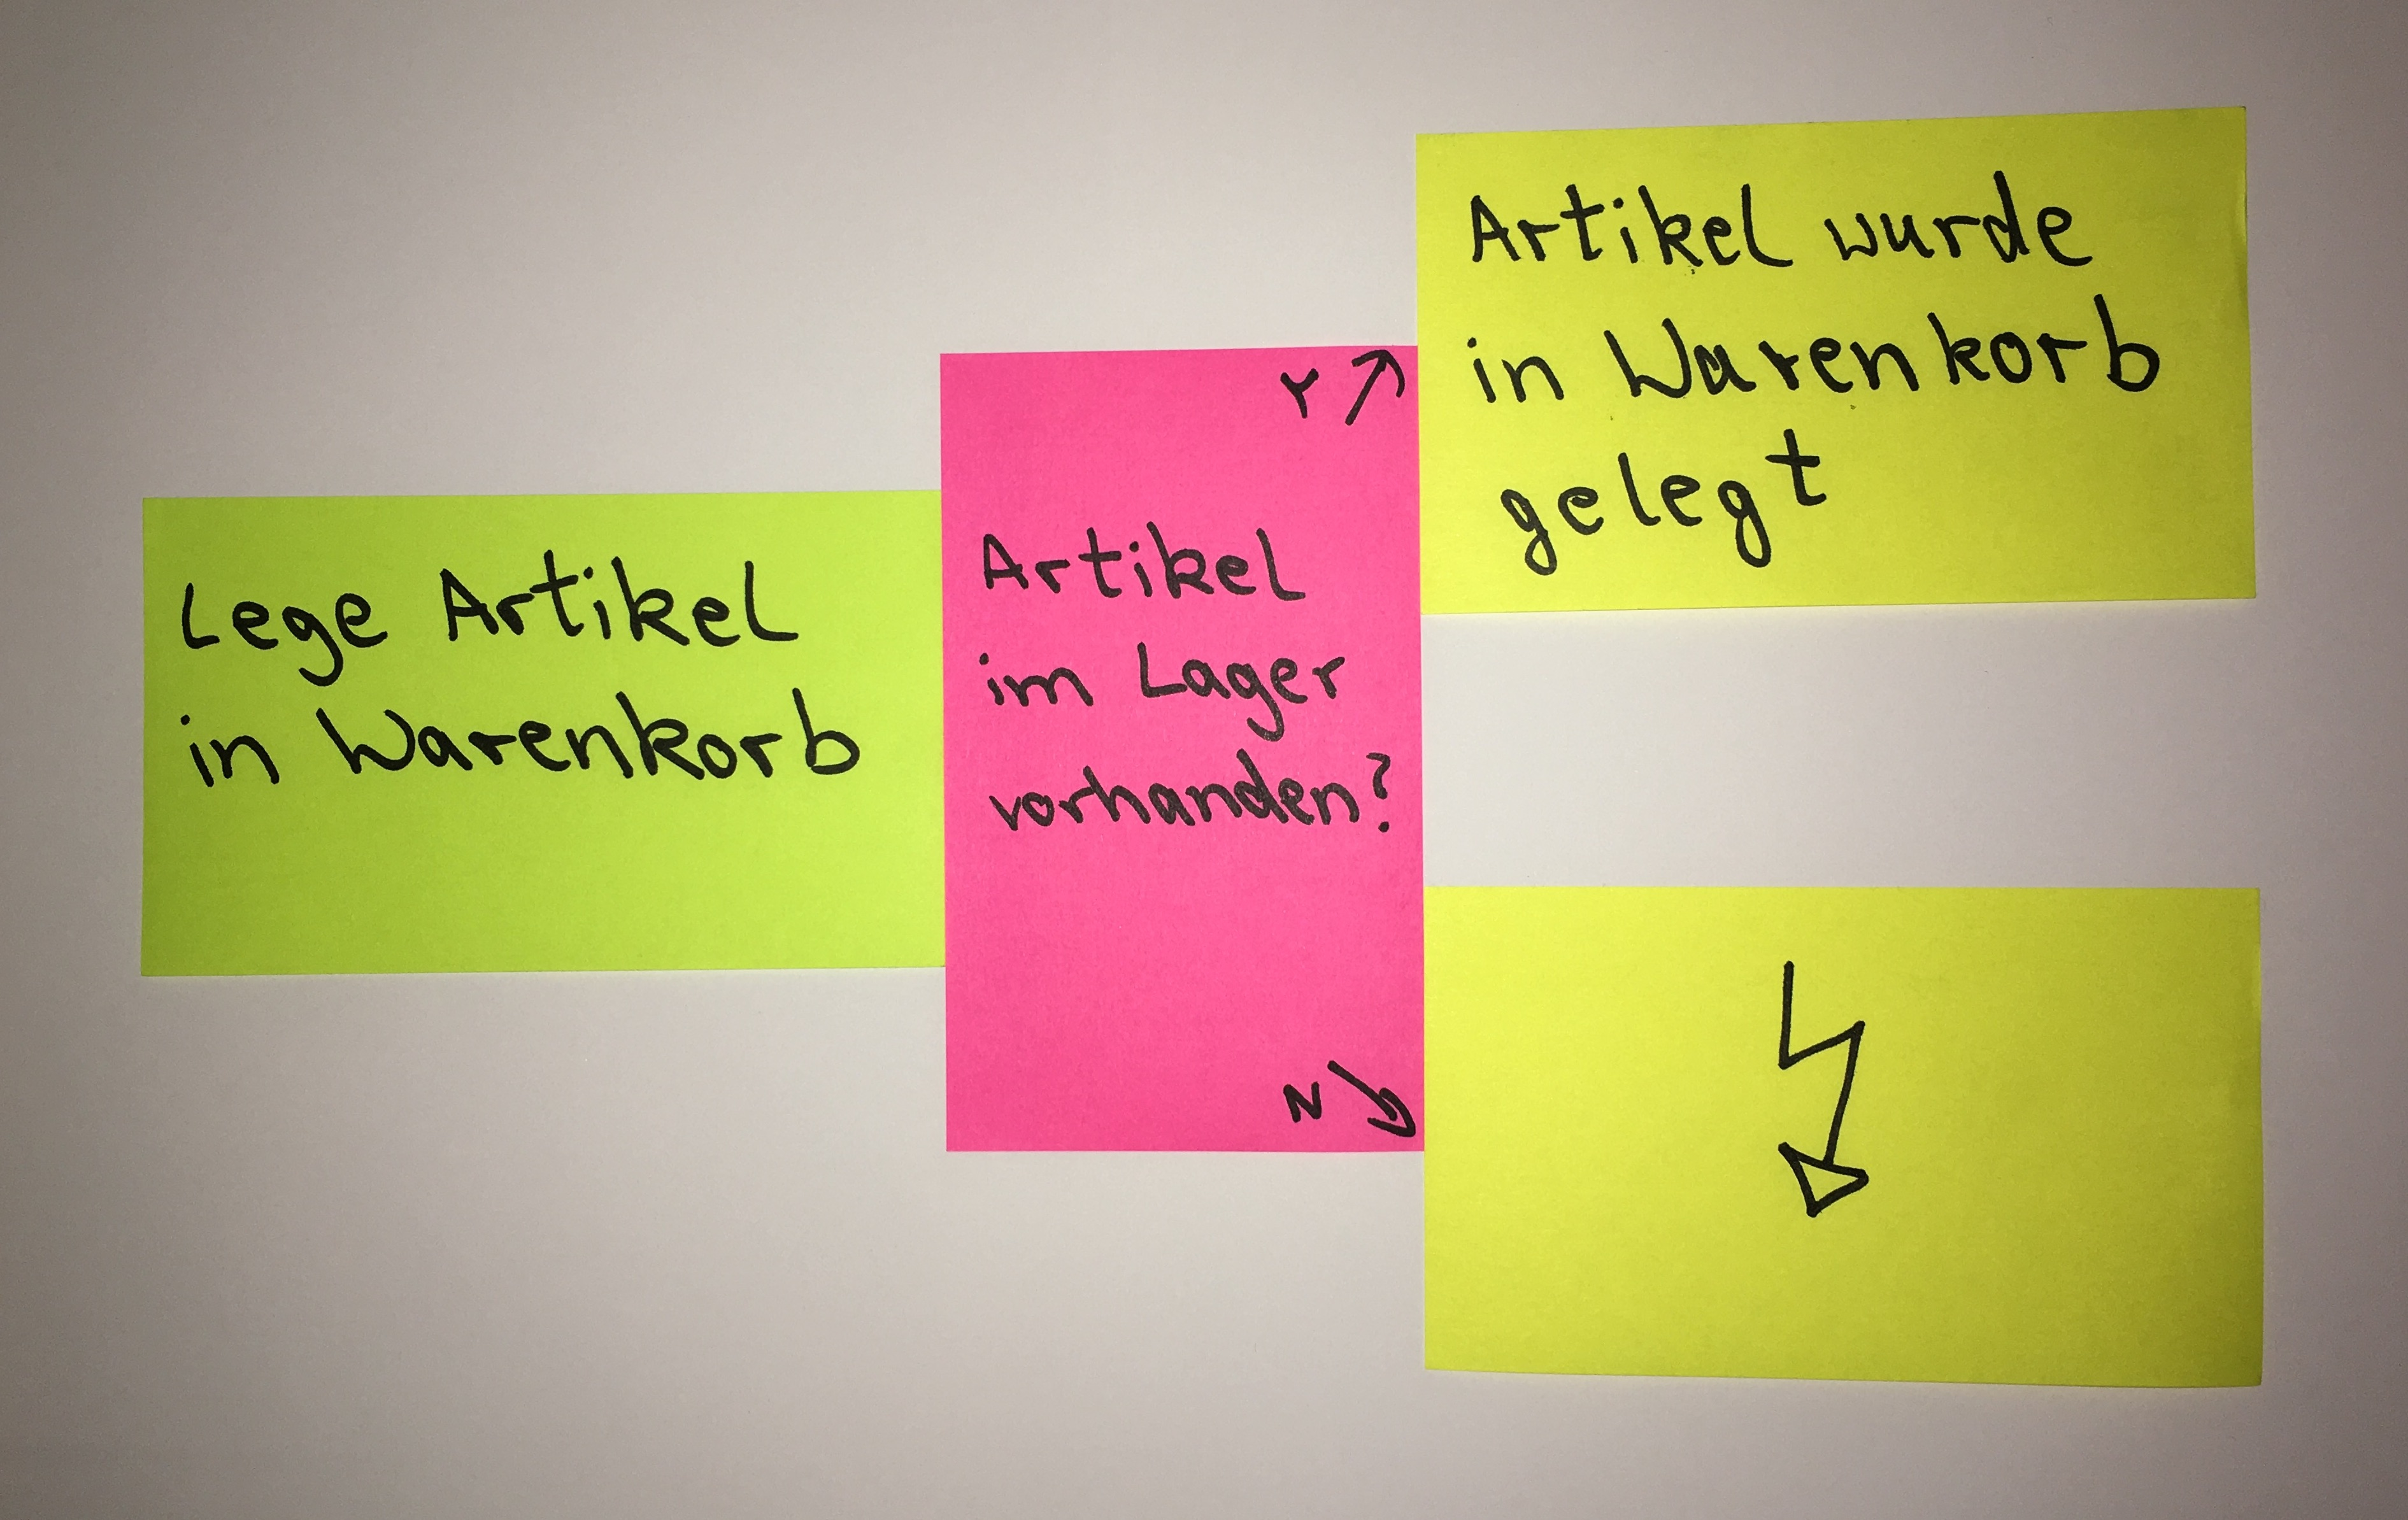
\includegraphics[width=.85\textwidth]{pics/eventstorming3.jpg}
\end{center}

\end{frame}

%-----------------------------------------------------------------------------------------------------------------------------------
\numberednote{

\textbf{Übung}

\begin{itemize}
\item Events um Commands und ggf.~auch Constraints ergänzen
\item Was musste passieren, damit dieses Event stattfinden konnte?
\item Sauberer modellieren
\item Clusterbildung
\item Granularität angleichen
\item Vollständigkeit checken, Fehlendes ergänzen
\end{itemize}

\hfill $\Longrightarrow$
}

\numberednote{
\textbf{Kritische Fragen:}

\begin{itemize}
\item Folgt dies immer direkt? 
\item Gibt es hier keine Constraints?
\end{itemize}

Wenn keine Constraints: Entweder Domäne langweilig oder Problem noch nicht verstanden

~\\
\textbf{Was kann schiefgehen?}

\begin{itemize}
\item x
\end{itemize}

}

%%%%%%%%%%%%%%%%%%%%%%%%%%%%%%%%%%%%%%%%%%%%%%%%%%
\begin{frame}[fragile]{\de{So kann das aussehen}\en{That's what it can look like}}

\begin{center}
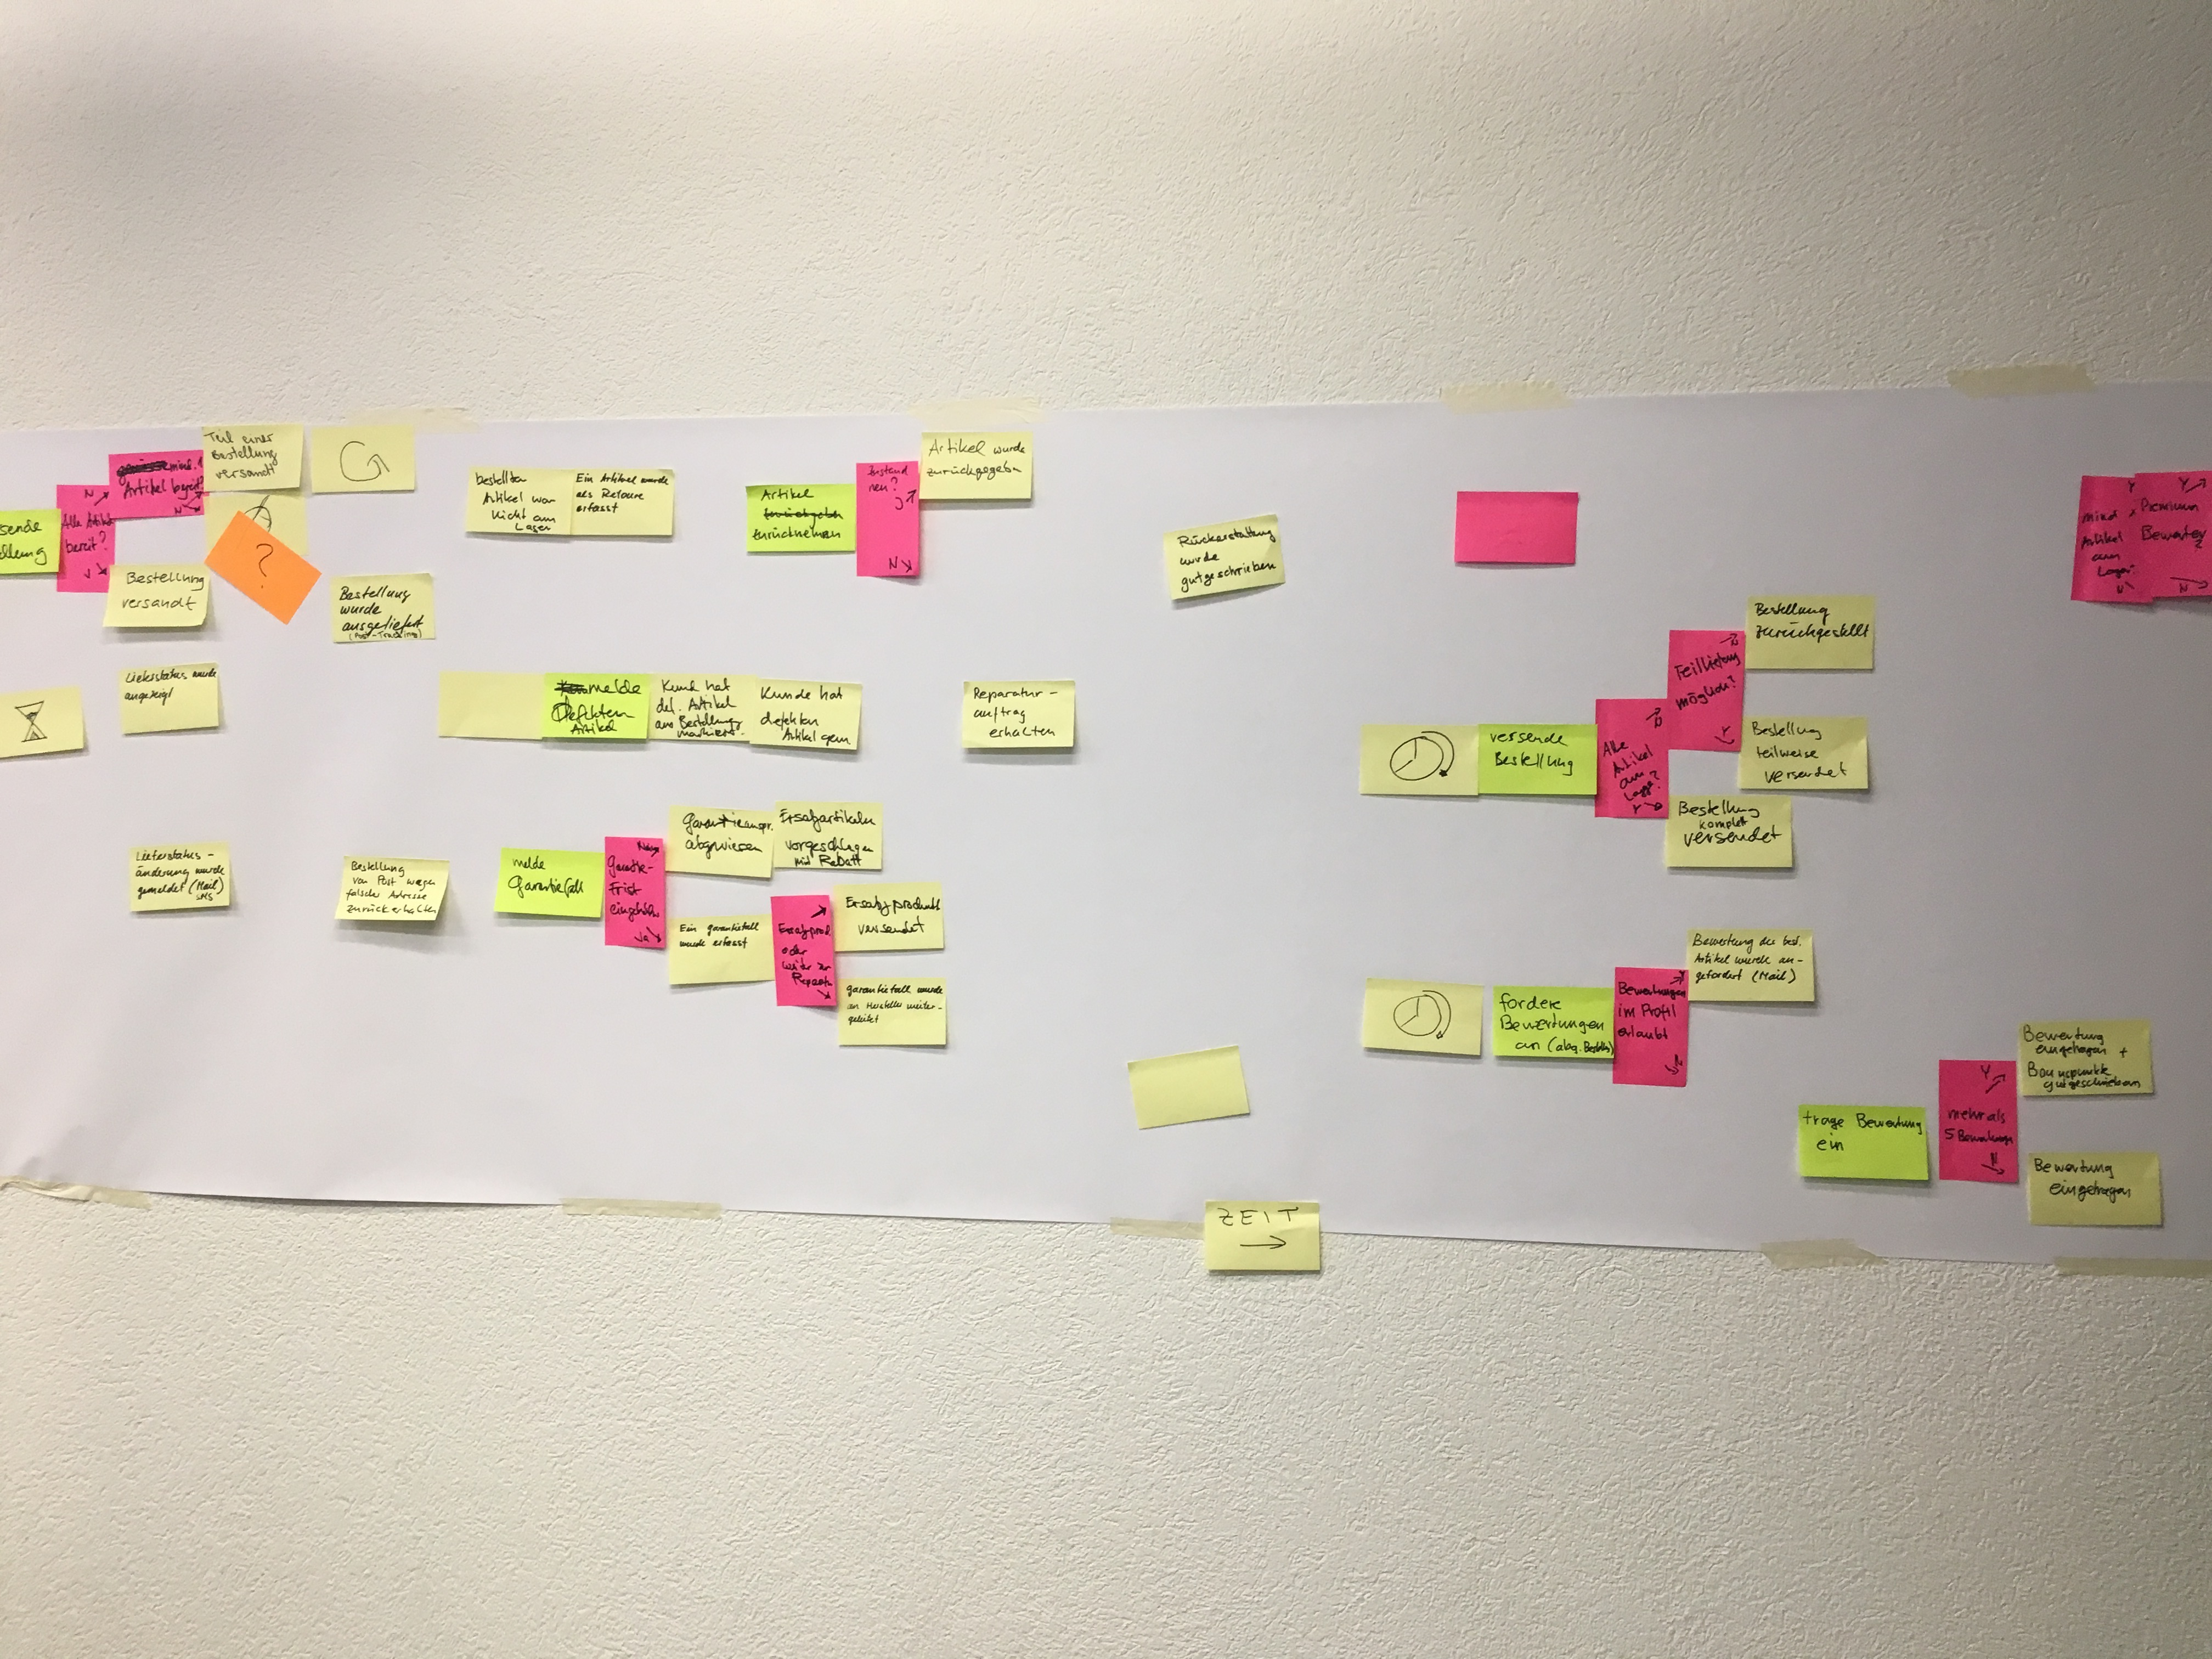
\includegraphics[width=.5\textwidth]{pics/modelling_commands_constraints1.jpg}
\end{center}

\end{frame}



%%%%%%%%%%%%%%%%%%%%%%%%%%%%%%%%%%%%%%%%%%%%%%%%%%
\begin{frame}[fragile]{\de{Darstellung von Zeit}\en{Representing Time}}

\onslide+<2->
 \begin{tikzpicture}
 % x (kleiner = weiter nach links) y (kleiner = weiter nach unten)
            \put (-10,-20) { 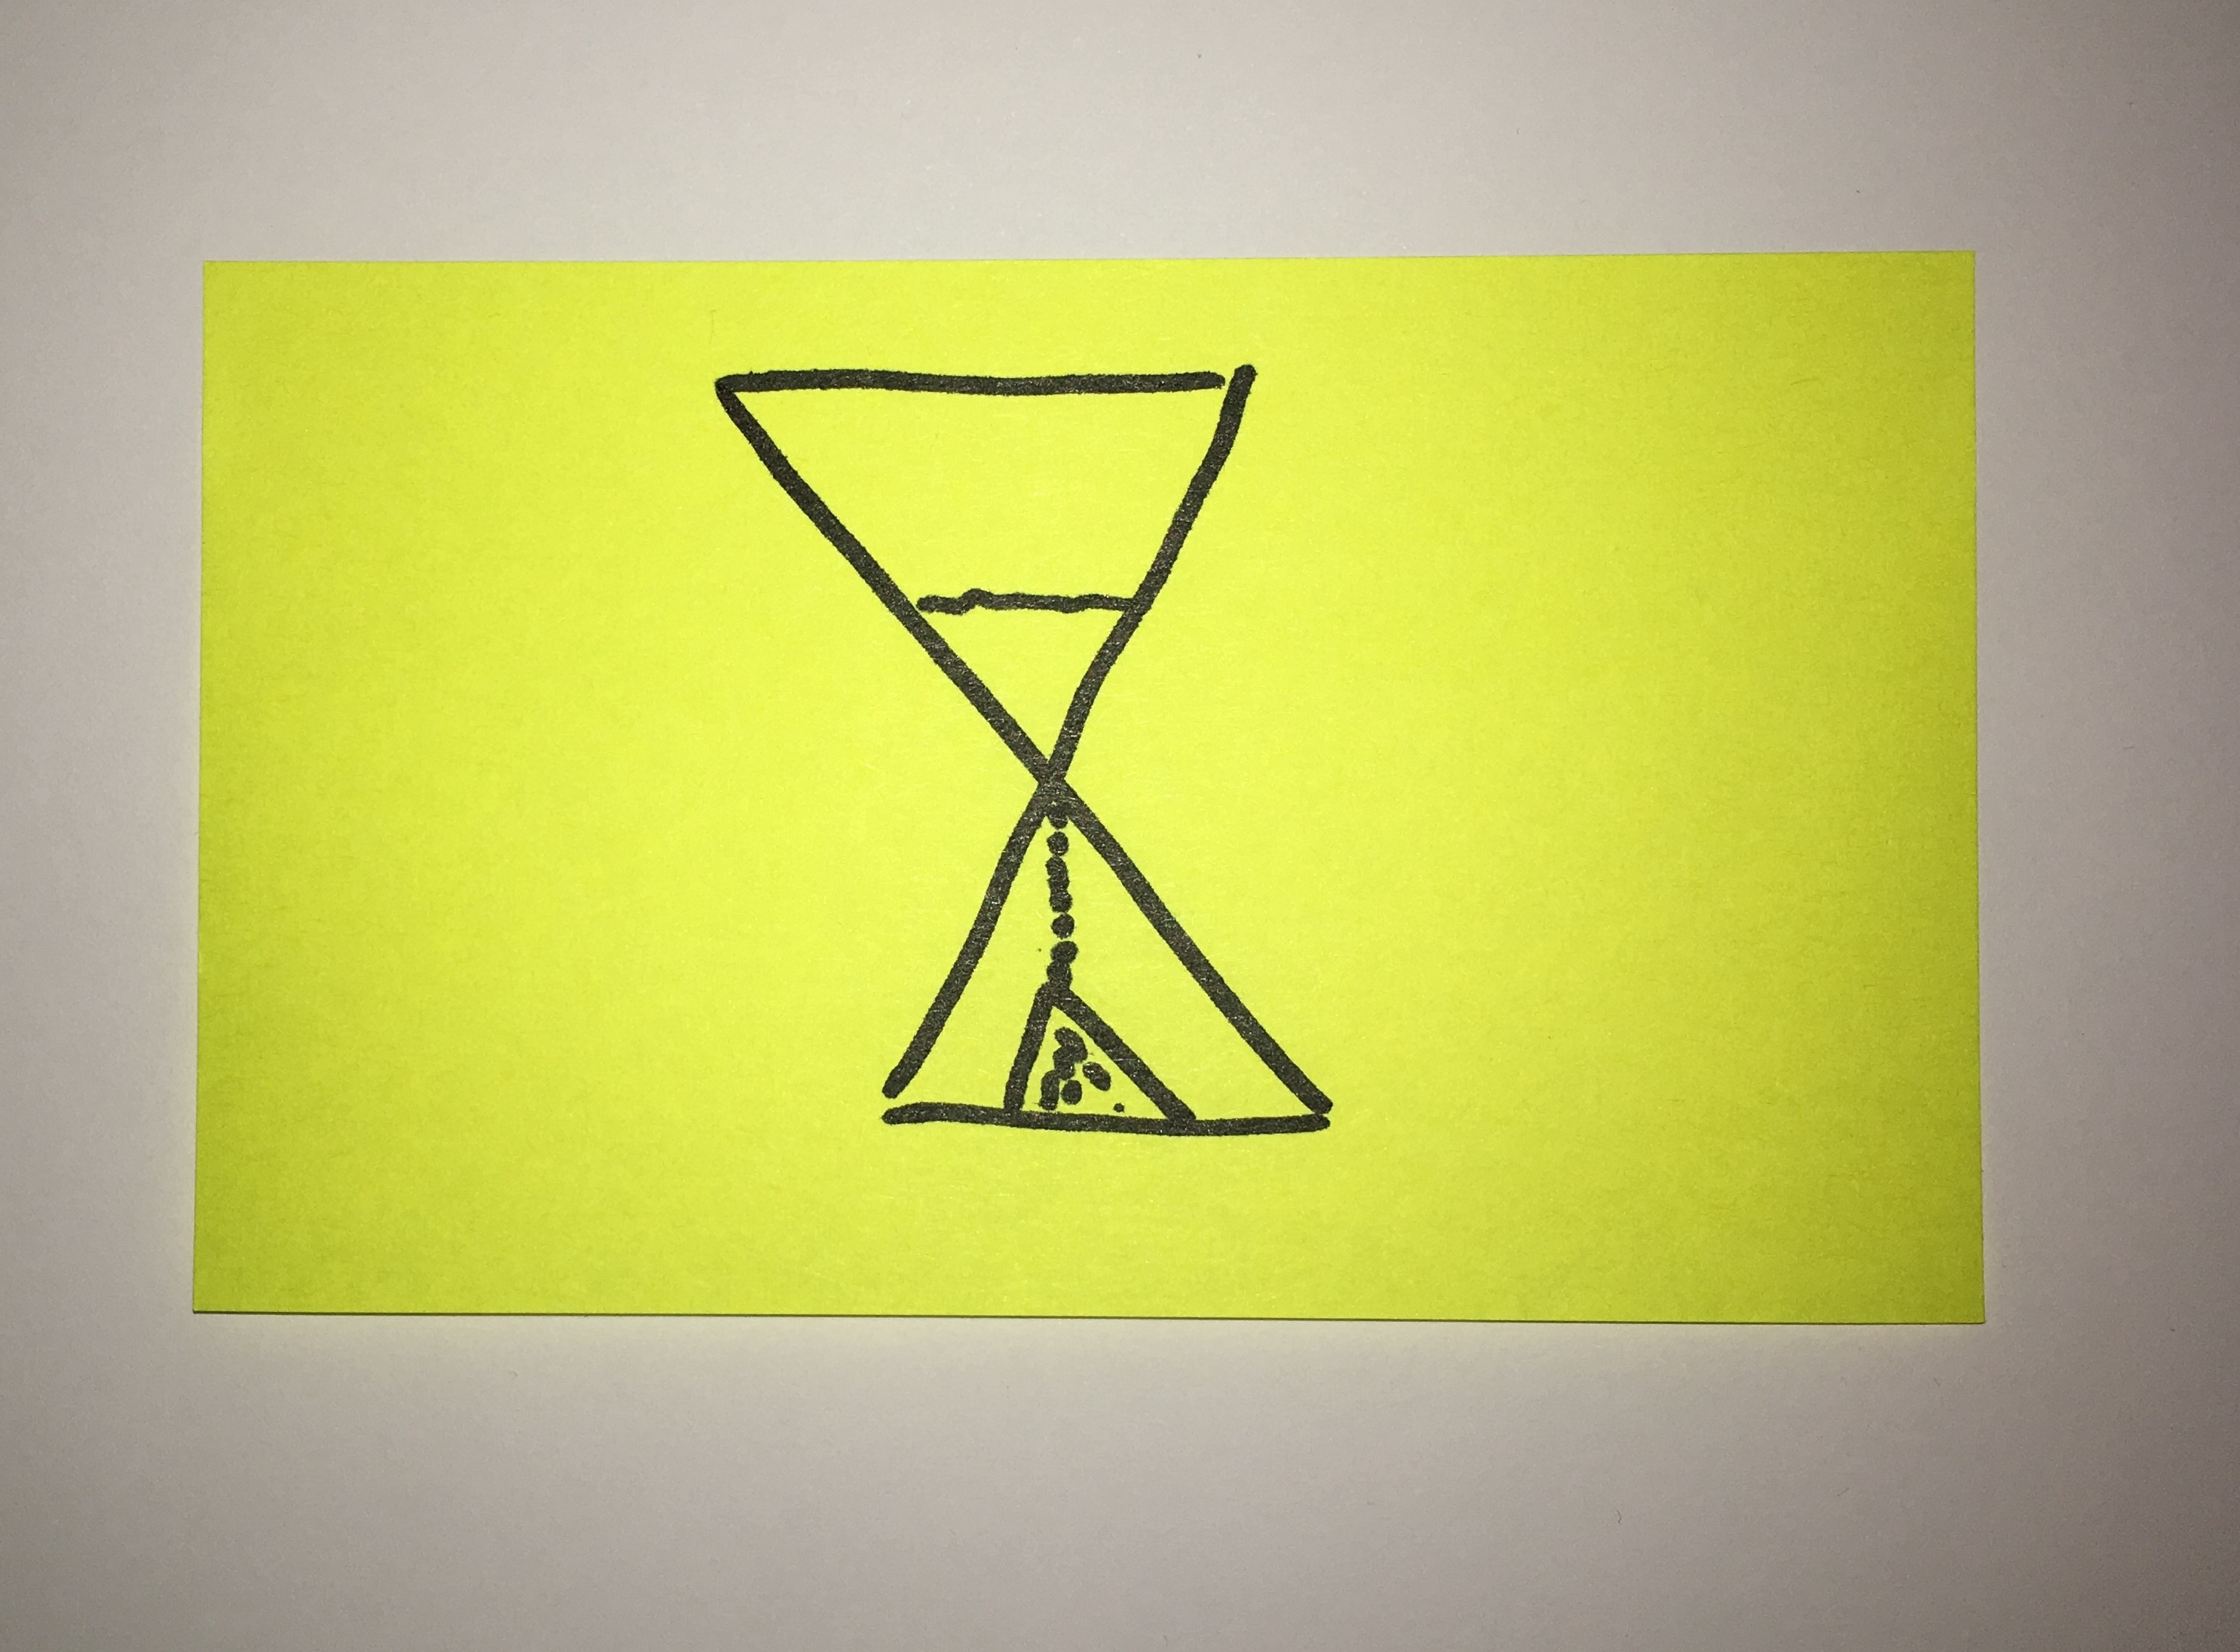
\includegraphics[width=.4\textwidth]{pics/darstellung_von_zeit_kurz.jpg} };
\end{tikzpicture}

\onslide+<3->
 \begin{tikzpicture}
            \put (150,-100) { 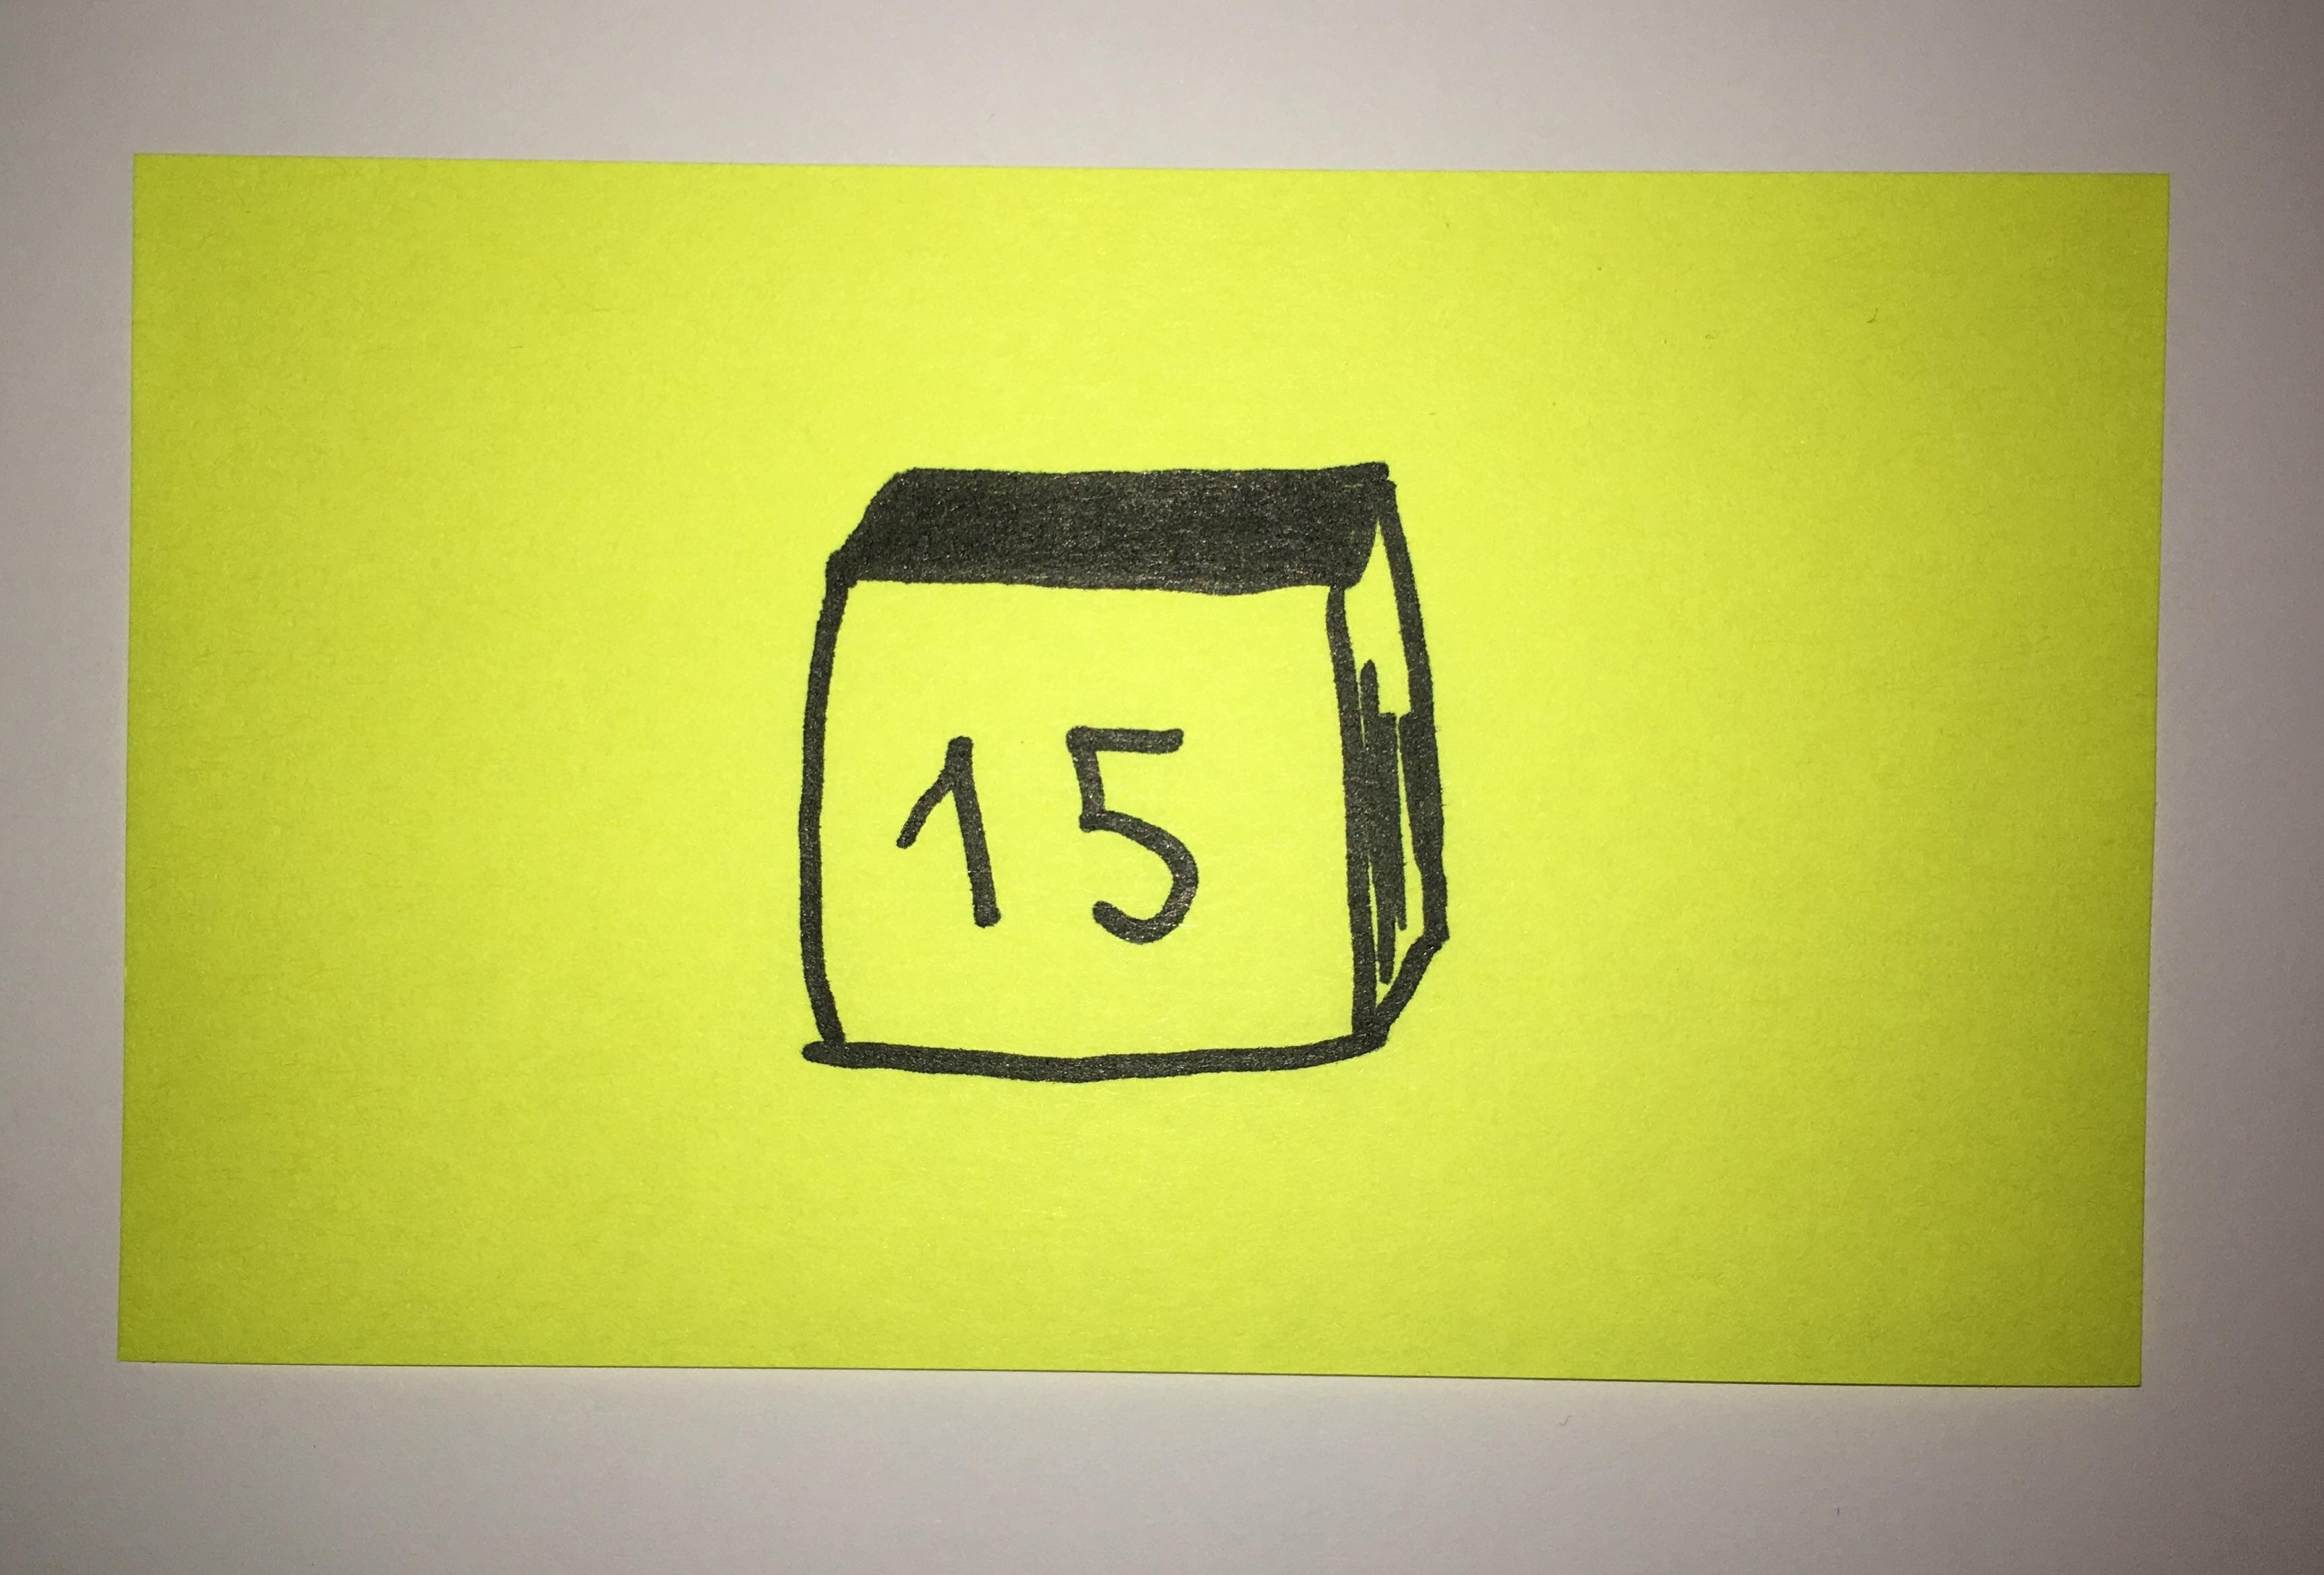
\includegraphics[height=.4\textheight]{pics/darstellung_von_zeit_lang.jpg} };
\end{tikzpicture}

\end{frame}

%%%%%%%%%%%%%%%%%%%%%%%%%%%%%%%%%%%%%%%%%%%%%%%%%%
\begin{frame}[fragile]{\de{Darstellung von Wiederholung}\en{Representing Repetition}}

\begin{center}

\includegraphics[width=.5\textwidth]{pics/darstellung_von_wiederholung.jpg}
\end{center}

\end{frame}

\numberednote{

Achtung: Entwickler denken gern in Wiederholungen = Schleifen

~\\

\textbf{Kritische Fragen:}

\begin{itemize}
\item Ist der nächste Durchlauf wirklich exakt identisch? 
\end{itemize}

Beispiel: Die 3. Mahnung sieht sicher anders aus als die erste...

}

%%%%%%%%%%%%%%%%%%%%%%%%%%%%%%%%%%%%%%%%%%%%%%%%%%
%%%%%%%%%%%%%%%%%%%%%%%%%%%%%%%%%%%%%%%%%%%%%%%%%%
\begin{frame}[fragile]{EventStorming IV}

\begin{itemize}
\item \de{Constraints benötigen \textbf{Daten} zur Entscheidung}\en{Constraints need \textbf{data} for their answers}
\item \de{Müssen verfügbar sein}\en{Data must be available}
\begin{itemize}
\item \de{Vorherige Erfassung in Event}\en{Captured via event before the command}
\item \de{Aus anderem Systemteil}\en{From another part of the system}
\end{itemize}
\item \de{Fehlen sie, muss das Modell ergänzt werden}\en{If missing $\Longrightarrow$ amend the model}
\end{itemize}

\end{frame}

%%%%%%%%%%%%%%%%%%%%%%%%%%%%%%%%%%%%%%%%%%%%%%%%%%
\begin{frame}[fragile]{\de{Beispiel}\en{Example}}

\begin{center}
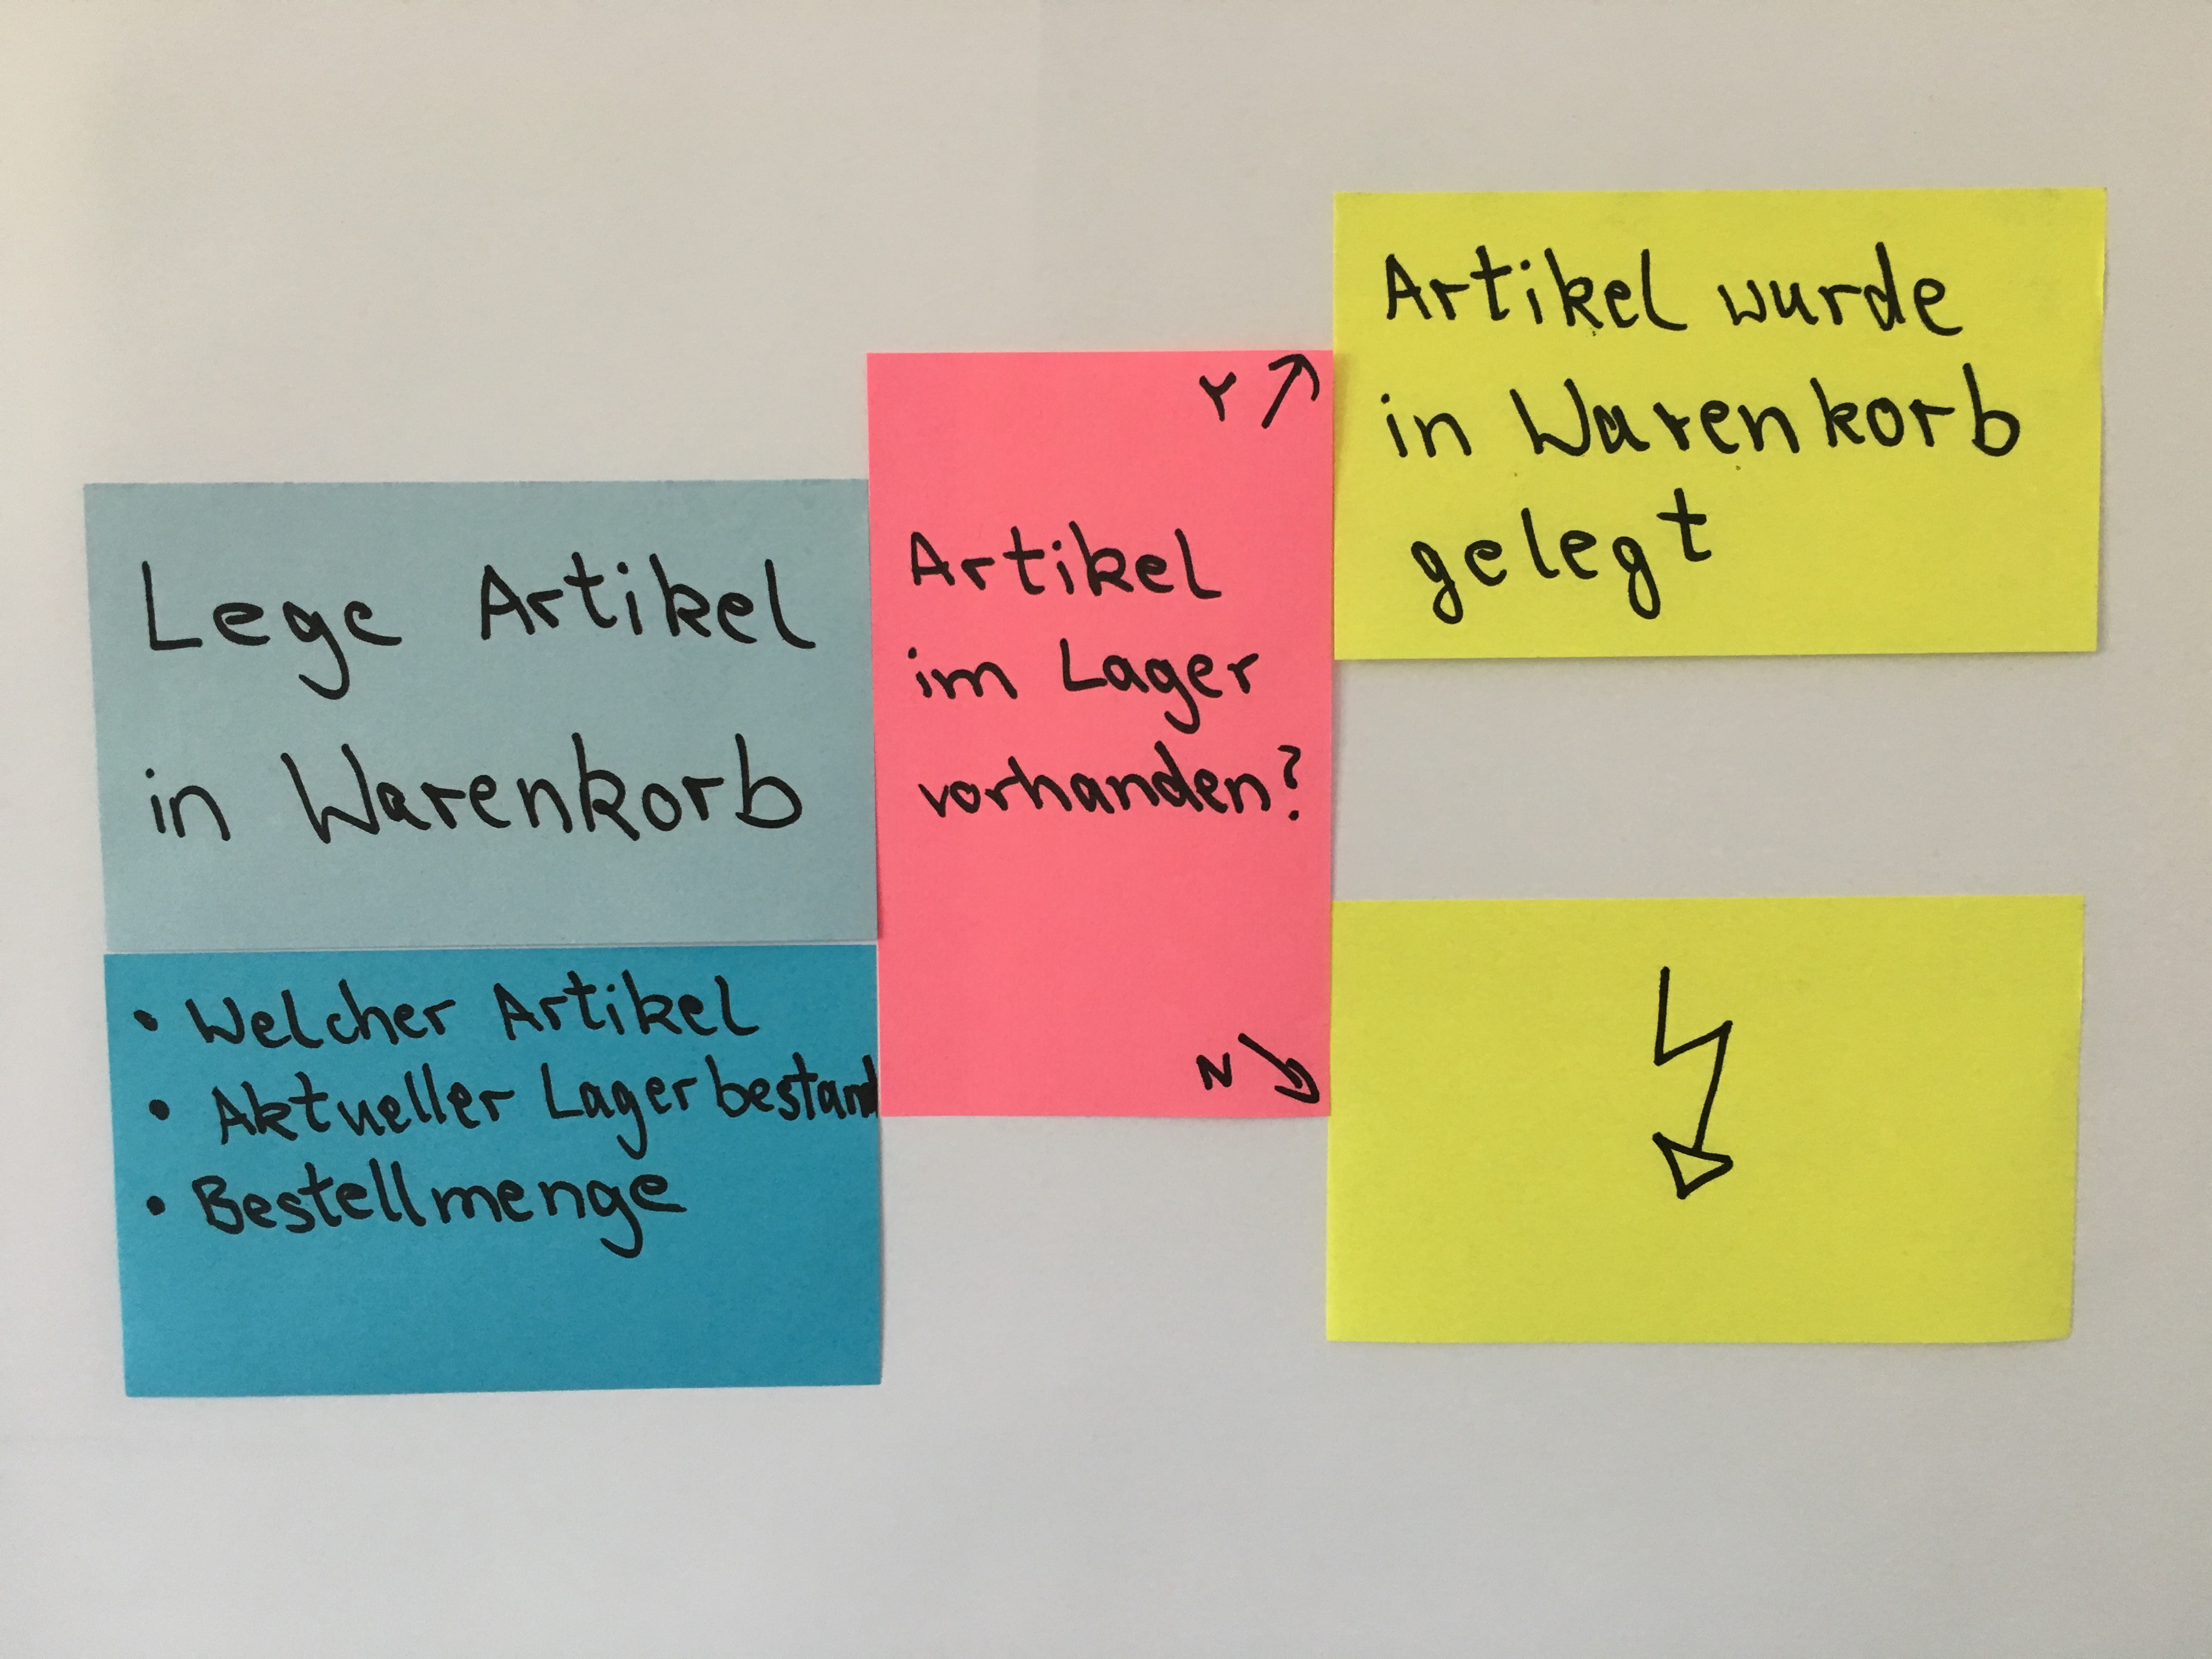
\includegraphics[width=.85\textwidth]{pics/eventstorming4.jpg}
\end{center}

\end{frame}

%-----------------------------------------------------------------------------------------------------------------------------------
\numberednote{

\textbf{Übung}

\begin{itemize}
\item In Constraints und Events erforderliche \textbf{Daten} zufügen
\item Fehlendes ergänzen
\item Datenquellen identifizieren
\item Verbindungen schaffen
\end{itemize}

~\\
\textbf{Kritische Fragen:}

\begin{itemize}
\item x
\end{itemize}

~\\
\textbf{Was kann schiefgehen?}

\begin{itemize}
\item x
\end{itemize}

}

%%%%%%%%%%%%%%%%%%%%%%%%%%%%%%%%%%%%%%%%%%%%%%%%%%
%%%%%%%%%%%%%%%%%%%%%%%%%%%%%%%%%%%%%%%%%%%%%%%%%%
\begin{frame}[fragile]{EventStorming V}

\begin{itemize}
\item \textbf{Bounded Contexts}
\begin{itemize}
\item \de{hohe Kopplung \textbf{innerhalb}}\en{high coupling \textbf{inside}}
\item \de{Wenige Abhängigkeiten \textbf{dazwischen}}\en{Few dependencies \textbf{across}}
\end{itemize}
\item \de{Abhängigkeiten ggf.~mit Wollfäden symbolisieren}\en{Can be modelled with yarn}
\end{itemize}

\end{frame}

%-----------------------------------------------------------------------------------------------------------------------------------
\numberednote{

\textbf{Übung}

Identifizieren Sie die Bounded Contexts in Ihrem Modell.

~\\
\textbf{Kritische Fragen:}

\begin{itemize}
\item x
\end{itemize}

~\\
\textbf{Was kann schiefgehen?}

\begin{itemize}
\item x
\end{itemize}

}

%%%%%%%%%%%%%%%%%%%%%%%%%%%%%%%%%%%%%%%%%%%%%%%%%%
%%%%%%%%%%%%%%%%%%%%%%%%%%%%%%%%%%%%%%%%%%%%%%%%%%
\begin{frame}[fragile]{EventStorming VI}

\begin{itemize}
\item \de{\textbf{Entwicklungspakete} (User Stories) ableiten}\en{Derive development units (user stories)}
\item \de{Command mit Events $\Rightarrow$ Story}\en{Command + events $\Rightarrow$ story}
\begin{itemize}
\item \de{Ggf.~aufteilen in Happy Path + weitere Fälle}\en{If necessary, split into Happy Path + further cases}
\end{itemize}
\end{itemize}

\end{frame}

%%%%%%%%%%%%%%%%%%%%%%%%%%%%%%%%%%%%%%%%%%%%%%%%%%
\begin{frame}[fragile]{\de{Beispiel}\en{Example}}

\begin{center}
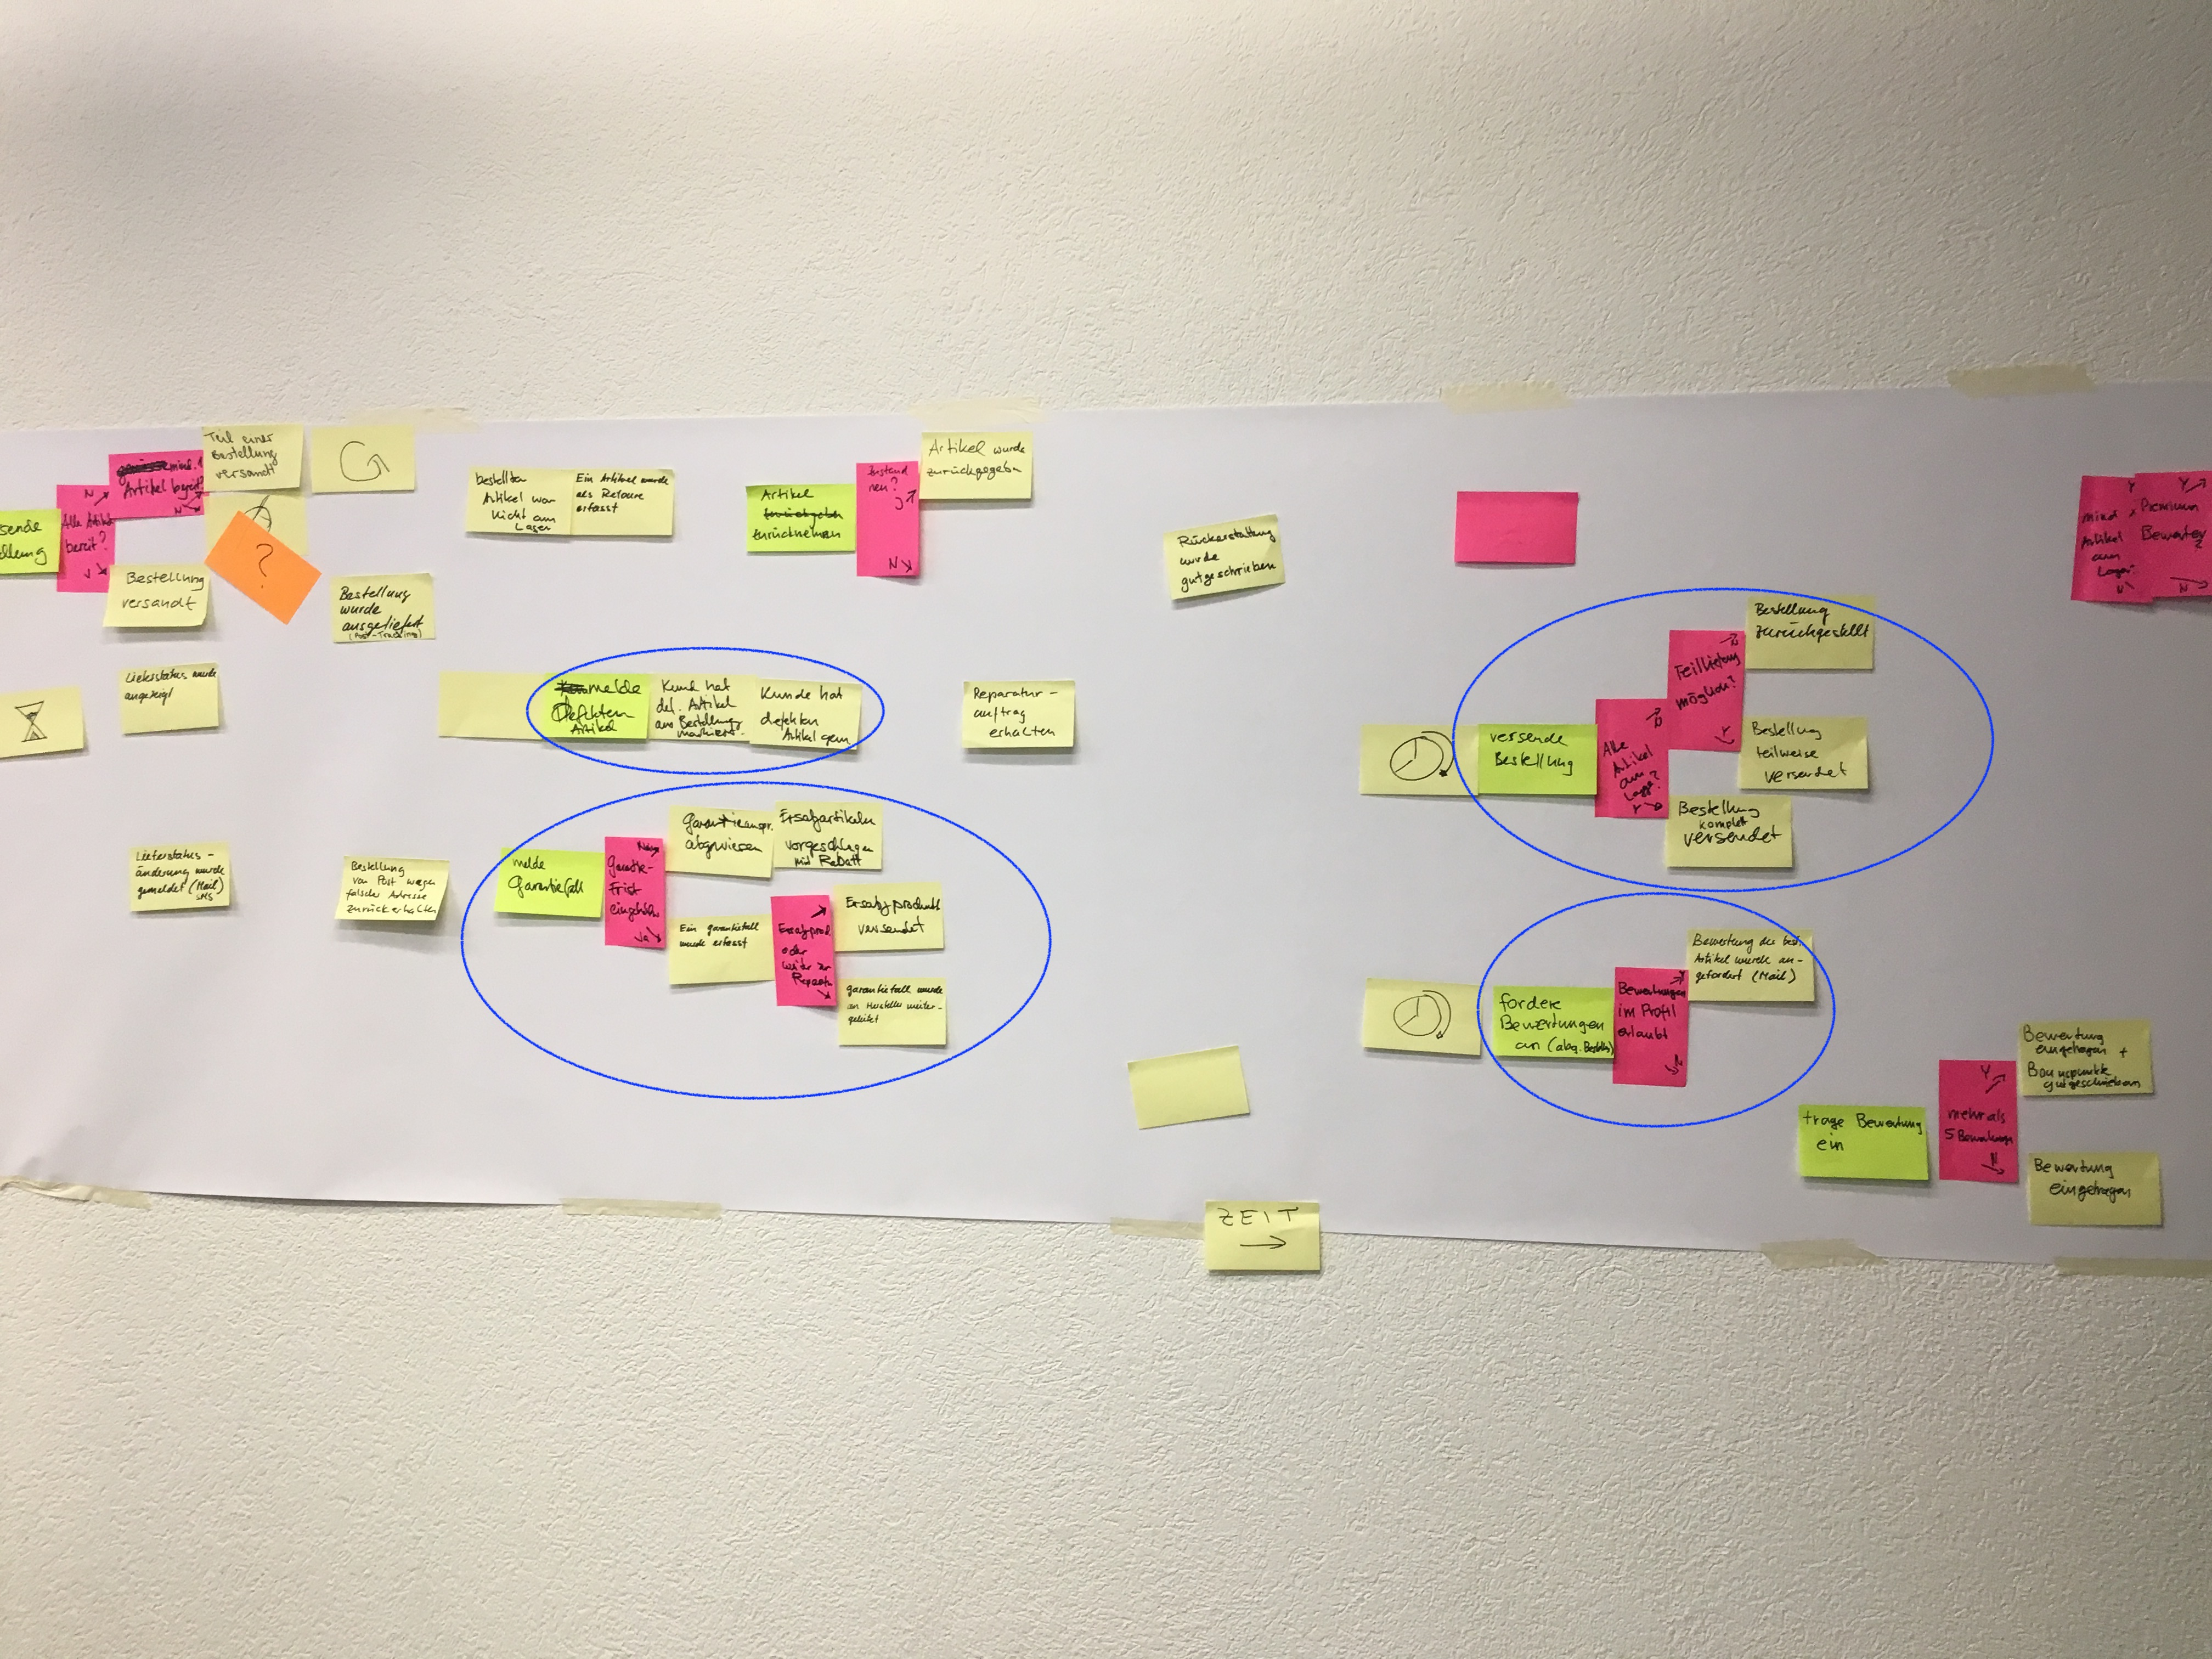
\includegraphics[width=.85\textwidth]{pics/eventstorming_stories.jpg}
\end{center}

\end{frame}

%-----------------------------------------------------------------------------------------------------------------------------------
\numberednote{

\textbf{Übung}

Identifizieren Sie User Stories in Ihrem Modell.

~\\
\textbf{Kritische Fragen:}

\begin{itemize}
\item x
\end{itemize}

~\\
\textbf{Was kann schiefgehen?}

\begin{itemize}
\item x
\end{itemize}

}


%%%%%%%%%%%%%%%%%%%%%%%%%%%%%%%%%%%%%%%%%%%%%%%%%%
%%%%%%%%%%%%%%%%%%%%%%%%%%%%%%%%%%%%%%%%%%%%%%%%%%
\begin{frame}[fragile]{\de{Wie geht es weiter?}\en{What's Next?}}

\de{Umsetzung einer Story:}\en{Implementing a story:}

\begin{itemize}
\item \de{Zuerst sehr detailliert modellieren, dann sofort implementieren}\en{Model in great detail, implement immediately}
\item \de{Modell an die Wand hängen während der Entwicklung}\en{Stick model to wall during development}
\item \de{Alle Diskussionen an und mit diesem Modell durchführen}\en{Discuss everything based on this model}
\item \de{Bei Änderungen Modell und Code aktualisieren!}\en{Changes $\Rightarrow$ update model and code!}
\item \de{Event Sourced Implementierung ist einfach realisierbar}\en{Easy to implement with event sourcing}
\end{itemize}

\end{frame}

%%%%%%%%%%%%%%%%%%%%%%%%%%%%%%%%%%%%%%%%%%%%%%%%%%
\begin{frame}[fragile]{}

\begin{center}
{
\LARGE
\de{Zusammenfassung}\en{Summary}
}
\end{center}

\end{frame}

%%%%%%%%%%%%%%%%%%%%%%%%%%%%%%%%%%%%%%%%%%%%%%%%%%
\begin{frame}[fragile]{\de{Warum Modellieren?}\en{Why Modelling?}}

\begin{itemize}
\item \de{Modellieren dient dazu, Gedanken sichtbar und \glqq begreifbar\grqq{} zu machen}\en{Modelling helps make thoughts visible and tangible}
\onslide+<2->
\item \de{Jeder entwickelt eigene Vorstellungen von etwas Gehörtem}\en{Everybody develops their own understanding of something they heard}
\onslide+<3->
\item \de{Ein Modell versucht Klarheit zu schaffen}\en{Model tries to add clarity}
\item \de{EventStorming ist ein Weg, sehr schnell zu einem sehr detaillierten Modell zu kommen}\en{EventStorming helps get to a detailed model in a very short period of time}
\end{itemize}

\end{frame}

%%%%%%%%%%%%%%%%%%%%%%%%%%%%%%%%%%%%%%%%%%%%%%%%%%
\begin{frame}[fragile]{\de{Kritische Fragen stellen}\en{Ask Critical Questions}}

\begin{itemize}
\item \de{Details mit dem Fachbereich abklären}\en{Clarify details with the business people}
\item \de{Das Modell kritisch hinterfragen!}\en{Critically question the model!}
\item \de{Modellierungs-Alternativen diskutieren!}\en{Discuss alternative models}
\item \de{\glqq Was wenn dies vor jenem passiert?\grqq}\en{``What if this happens earlier than that?''}
\item \de{Die üblichen Verdächtigen (\glqq immer\grqq, \glqq nie\grqq, \glqq kann nicht sein\grqq{} \ldots) verfolgen und entkräften}\en{Follow the Usual Suspects$^{\textsf{TM}}$ (\textit{always, never,} ...) and invalidate them}
\end{itemize}

\end{frame}

%%%%%%%%%%%%%%%%%%%%%%%%%%%%%%%%%%%%%%%%%%%%%%%%%%
\begin{frame}[fragile]{\de{Einsichten in die Domäne gewinnen}\en{Gain Insights into the Domain}}
\begin{itemize}
\item \de{Kollaboration zwischen Fachbereich und Entwicklern ist der entscheidende Faktor für den Erfolg eines Projekts}\en{Collaboration between devs and business is key for a project's success}
\item \de{Man braucht die Domänen-Experten des betreffenden Bereiches}\en{You need your domain experts}
\item \de{EventStorming ist auch ohne DDD einsetzbar}\en{EventStorming can be used without DDD}
\end{itemize}

\end{frame}

